%\chapter{Часть вторая. Объектно-ориентированное программирование в \Sys{C++}}
\renewcommand{\arraystretch}{0.5}
\chapter{Объектно-ориентированное программирование}%Возникновение объектного подхода в программировании}
\section{Возникновение объектного подхода в программировании}
Первые программы, создававшиеся в те времена, когда значения битов в регистрах переключались тумблерами на системной
консоли и тут же отображались загорающимися индикаторами --- эти первые программы были чрезвычайно просты. Писали их
непосредственно в машинных кодах, или, в лучшем случае, на ассемблере --- языке, заменяющем коды машинных команд
буквенными мнемониками. В последствии, по мере усложнения компьютеров и увеличения размеров программ, отслеживать
возникающие ошибки становилось всё труднее. Поэтому стала возрастать популярность языков программирования высокого
уровня, а число программ, написанных целиком на языке машинных команд, наоборот, начало сокращаться. Языки высокого
уровня обеспечивали более высокий уровень абстракции, приближая конструкции и операторы языка к понятиям, которыми
оперирует человек.

Исторически одним из первых языков высокого уровня был Фортран, завоевавший огромную популярность и до сих пор
используемый иногда в научных и инженерных расчётах. Подход к программированию, на котором был основан и он, и многие
другие ранние языки, получил название \emph{процедурного программирования}. В рамках этого подхода в
программе отдельно хранятся \emph{процедуры} --- блоки кода, каждый из которых выполняет какое-то
самостоятельное действие, и \emph{переменные} --- блоки данных (см. рис.~\ref{ch10:refDrawing0}), к которым
обращаются процедуры для получения исходных значений и для сохранения результата. Такая чётко структурированная
программа создавала меньше возможностей не заметить ошибку. Поэтому производительность труда программистов, освоивших
процедурную парадигму, ощутимо вырастала, а вместе с производительностью труда вырастали размеры программ и их
функциональные возможности. Код серьёзных программных продуктов всё чаще писался коллективно, и скоро процедурный
подход перестал казаться таким уж защищённым от ошибок. Например, нередко возникали ситуации, когда несколько
программистов одинаково называли свои переменные, т.~е. фактически использовали одну и ту же глобальную переменную в
разных целях, в результате чего её значение хаотично менялось при вызове разных процедур. 

\begin{figure}[htb]
\begin{center}
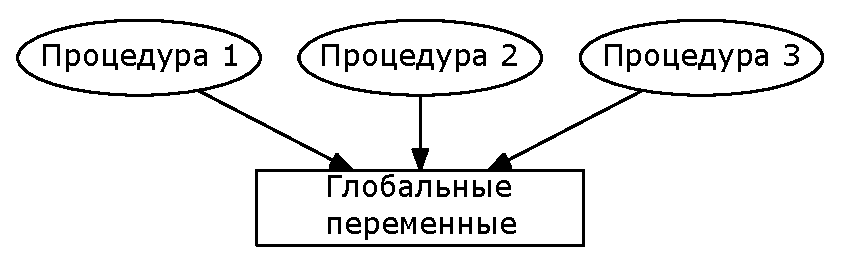
\includegraphics[width=0.5\textwidth]{img/ris_10_1}
\caption{Процедурный подход к программированию}
\label{ch10:refDrawing0}
\end{center}
\end{figure}



Процедурный подход претерпел ряд модернизаций, более современные языки высокого уровня заимствовали некоторые принципы
\emph{функционального программирования} (одним из удачных примеров такого симбиоза является язык \Sys{C}),
большие программы делились на модули, а фирмы вводили собственные строгие политики в области оформления программного
кода. Но в большой программе по-прежнему было слишком трудно разобраться и слишком просто запутаться, поэтому проблема
всё равно оставалась.

\emph{Объектный подход} родился как следующий важный шаг на пути качественного написания больших программ.
В нём предлагается разделять программу на самостоятельные части --- \index{Объект}\emph{объекты}, наделённые
собственными свойствами, текущим состоянием, и умеющие взаимодействовать друг с другом и с окружающей средой --- примерно
так, как это происходит у объектов реального мира.

В упрощённом виде такая парадигма получила название объектно-ориентированного программирования (ООП) --- подхода, который
позволяет использовать в программе объекты и даже поощряет эту практику, но не требует, \emph{чтобы
программа состояла из одних только объектов}.

Классическое определение объекта звучит следующим образом:

\emph{Объект --- это осязаемая сущность, которая чётко проявляет своё поведение.}

Читателю, для которого объектный подход к программированию внове, такое определение наверняка покажется слишком
туманным. Позже конкретные примеры прояснят  ситуацию, а пока поговорим о внутреннем устройстве объекта.

Объект состоит из следующих трёх частей:

\begin{itemize}
\item имя объекта;
\item состояние (переменные состояния);
\item методы (операции).
\end{itemize}

На рисунке~\ref{ch10:refDrawing1} изображены два объекта с именами <<Объект 1>> и <<Объект 2>>. Первый объект имеет две
переменные состояния и три метода, в то время как второй объект обходится одной единственной переменной состояния и
двумя методами.

\begin{figure}[htb]
\begin{center}
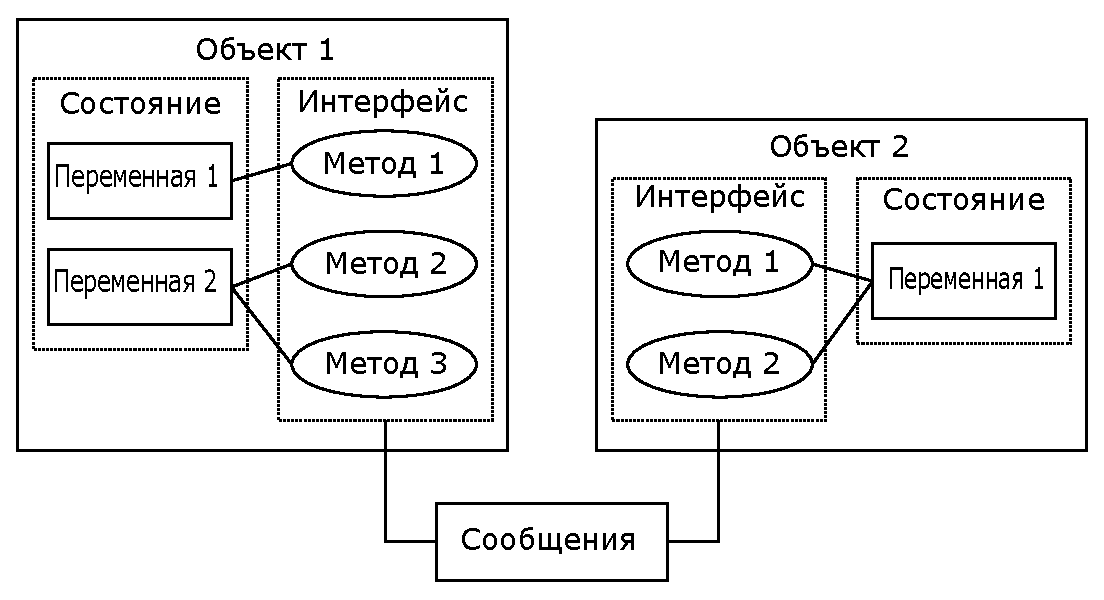
\includegraphics[width=0.7\textwidth]{img/ris_10_2}
\caption{Объектный подход к программированию}
\label{ch10:refDrawing1}
\end{center}
\end{figure}


Интерфейс объекта с окружающей средой (пользователем, остальной частью программы, операционной системой и т.~д.)
полностью осуществляется методами: к состоянию объекта нет другого доступа извне, кроме как через его методы. Например,
если объект должен передавать окружающей среде информацию о значении одной из своих переменных состояния --- для этого
создают специальный метод.

Закрытость внутреннего состояния объекта от окружающей среды известна также как свойство
\index{Объект!инкапсуляция}\emph{инкапсуляции}. Инкапсуляция означает, что объект содержит внутри себя данные и
методы, оперирующие этими данными. Фактически, для окружающей среды объект представляет собой аналог <<чёрного ящика>>:
принимает входные воздействия и выдаёт в качестве реакции на них выходные, но при этом никак не проявляет свою
внутреннюю структуру.

Для взаимодействия друг с другом объекты обмениваются \emph{сообщениями}, причём объект, получивший
сообщение, может либо проигнорировать сообщение, либо выполнить содержащуюся в нём команду (с помощью какого-либо из
своих методов).

Однотипные объекты образуют \index{Класс}\emph{класс}. Под однотипными объектами мы понимаем такие объекты,
у которых одинаковы наборы методов и переменных состояния. При этом объекты, принадлежащие одному классу, имеют разные
имена и, вероятно, разные значения переменных состояния. Например, можно придумать класс <<студент>>, объектами которого
будут конкретные студенты вуза. Объект класса <<студент>> должен иметь переменные состояния, в которых содержится
информация о конкретном студенте: Ф.И.О., номер студенческой группы, домашний адрес, список изучаемых дисциплин и т.~д.
Конкретный список переменных зависит от задачи, для решения которой создаётся программа. Так, если поставлена задача
автоматизировать работу университетской библиотеки, то объекты класса <<студент>> определённо должны содержать информацию
о книгах, взятых на абонемент конкретным студентом. Если автоматизируется учёт успеваемости, то в списке книг нет
необходимости, но зато в состояние объекта обязательно должны быть включены оценки по изучаемым дисциплинам.

Более того, когда мы рассматриваем сущности реального мира, с которыми должна иметь дело создаваемая программа, мы можем
назначить некую сущность на роль объекта или на роль класса объектов, также в зависимости от конкретной задачи.
Представим себе, что одна из подзадач программы --- систематизировать социальные роли, такие как <<домохозяйка>>,
<<пенсионер>>, <<студент>> (например, для учёта доходов и льгот). Вполне вероятно, что в такой программе <<социальная роль>>
будет объявлена классом, а сущность <<студент>> будет всего лишь одним из объектов. 

Иными словами, нет одинакового для всех ситуаций правила, по которому сущность делают объектом или классом объектов.
Всегда необходимо исходить из большей целесообразности. 

В реальном мире из родственных по смыслу сущностей часто можно составить иерархию <<от общего к частному>>. Такие
отношения в объектно-ориентированном подходе называются
\index{Класс!наследование}\emph{наследованием}. Из двух классов,
находящихся в отношении наследования, более общий класс называется
\index{Класс!базовый}\emph{базовым} или
\index{Класс!родительский}\emph{родительским} классом, а класс, представляющий собой более
частный случай, называется \index{Класс!дочерний}\emph{дочерним} или
\index{Класс!производный}\emph{производным} классом. Производный класс может заимствовать
атрибуты (свойства и методы) базового класса. Это означает, что если в программе используются родственные по смыслу
классы, обладающие некоторыми одинаковыми свойствами и методами --- лучше определить один базовый класс, находящийся в
вершине иерархии, и разместить дублирующиеся свойства и методы в нём. В этом случае производные классы смогут
автоматически унаследовать эти атрибуты от базового класса, и поэтому их не придётся описывать снова и снова. Например,
если программа оперирует классами <<студент>>, <<преподаватель>> и <<инженер>>, логично ввести дополнительный базовый класс
<<человек>>, переместив в него атрибуты, содержащие имя, адрес, другие личные данные, а также методы, манипулирующие
этими данными.

Помимо двух уже рассмотренных качеств --- инкапсуляции и наследования --- у объектов есть ещё третье основополагающее
качество: \index{Объект!полиморфизм}\emph{полиморфизм}. Это означает, что объекты  могут вести себя
по-разному в зависимости от ситуации. Одно из основных проявлений полиморфного поведения --- перегрузка функций. Объект
может содержать в себе несколько методов с одинаковыми именами, принимающих разные наборы параметров. В результате,
передавая объекту данные, можно обращаться к одному и тому же имени метода, не заботясь о типе, в котором представлены
данные. Правильно сконструированный объект автоматически выполнит наиболее подходящий метод из группы.

Инкапсуляция, наследование и полиморфизм являются тремя основополагающими принципами объектно-ориентированного
программирования и в том или ином виде реализуются во всех объектно-ориентированных языках. В следующих разделах мы
увидим, как конкретно эти принципы применены в \Sys{C++}.

\section[Классы и объекты в \Sys{C++}]{Классы и объекты в \Sys{C++}}
Хотя \Sys{C++} и не первая попытка создать объектно-ориентированную версию языка \Sys{С}, среди попыток такого рода он оказался
наиболее успешным. Очевидно, одна из причин успешности --- то, каким образом объектная парадигма была встроена в
синтаксис языка. 

Ранние версии \Sys{C++} были созданы в начале 1980-х Бьёрном Страуструпом для собственных нужд (в качестве универсального
языка программирования, удобного для компьютерного моделирования). В создаваемый язык были заложены следующие основные
принципы:

\begin{itemize}
\item поддержка различных стилей программирования, включая процедурный и объектно-ориентированный подходы;
\item предоставление программисту полной свободы выбора --- в т.~ч. реализовать программные решения, которые могут
казаться концептуально неверными;
\item сохранение обратной совместимости с языком С, чтобы программист мог использовать только те дополнительные
возможности \Sys{C++}, которые он сочтёт нужным, или не использовать их вовсе;
\item сохранение переносимости и высокой производительности, характерных для языка \Sys{С}.
\end{itemize}
Эти принципы заслужили высокую оценку программистов-практиков. В результате на текущий момент \Sys{C++} является одним из
наиболее распространённых языков программирования --- как системного, так и прикладного. 

\subsection[Реализация ООП в \Sys{C++}. Классы и структуры]{Реализация ООП в \Sys{C++}. Классы и структуры}
Синтаксис описания класса во многом копирует синтаксис описания структуры. В простейшем случае класс описывается  так:
\begin{lstlisting}
class `\Sys{имя\_класса}` 
{
  `\Sys{закрытые члены класса}`
  public:
  `\Sys{открытые члены класса}`
};
\end{lstlisting}

Как и при объявлении структуры, \Sys{имя\_класса} становится новым именем типа данных, которое можно
использовать для объявления переменных (объектов класса)~\cite{OOP,OOPz}. %[5,6]. 
Членами класса будут переменные и функции, объявленные
внутри класса. Функции-члены класса называют \emph{методами} этого класса, а переменные-члены класса
называют \emph{свойствами} класса.

В \Sys{C++} понятия ООП используются следующим образом~\cite{OOP,OOPz}: %[5,6]:

\begin{itemize}
\item <<\emph{класс}>>: пользовательский тип данных, во многом аналогичный  структуре;
\item <<объект класса>> или <<\emph{переменная-экземпляр класса}>>: переменная, в описании которой какой-то
класс указан в качестве типа данных;
\item \index{Класс!свойство}<<\emph{свойство}>> или <<\index{Класс!переменная-член
класса}\emph{переменная-член класса}>>: переменная, объявленная внутри класса (как поле внутри структуры);
на практике чаще говорят не о свойстве класса, а о \emph{свойстве объекта}, так как для конкретных
объектов переменные --- члены класса обладают конкретными значениями и потому имеют конкретный смысл.
\item <<\index{Класс!метод}\emph{метод}>>: функция, объявленная внутри класса.
\end{itemize}
По умолчанию все функции и переменные, объявленные в классе, являются \emph{закрытыми}, т.~е. принадлежат
\emph{закрытой секции класса.} Это значит, что они доступны для обращения только изнутри членов этого класса и
недоступны извне. Для объявления \emph{открытых} членов класса используется ключевое слово
\Sys{public} с двоеточием, обозначающее начало \emph{открытой секции класса}. Все члены
класса, объявленные после слова \Sys{public}, доступны для обращения как изнутри этого же класса, и для
любой другой части программы, в которой доступен класс. 

Открытых и закрытых секций в классе может быть несколько, и они могут произвольно чередоваться. При необходимости
обозначить очередную закрытую секцию, её начало обозначается ключевым словом \Sys{private}.

Более того, структуры в \Sys{C++} были существенно доработаны (по сравнению с  классическим вариантом 
структур языка \Sys{С}). 
В \Sys{C++}
структура может иметь помимо переменных-членов (т.~е. полей структуры) также и функции-члены, а ещё в структурах можно
вводить открытые и закрытые секции. В сущности, структуры отличаются от классов двумя вещами:

\begin{itemize}
\item в структурах вместо ключевого слова \Sys{class} пишется ключевое слово
\Sys{struct};
\item в структурах по умолчанию все члены являются отрытыми (иначе перестали бы работать программы, написанные на \Sys{С}). 
\end{itemize}
Рассмотрим в качестве примера объект, представляющий собой геометрический вектор в трехмерном пространстве. Для простоты
ограничимся хранением в объекте трёх координат и функции, вычисляющей модуль вектора. С учётом различий между
структурами и классами, приведённые ниже варианты аналогичны.
\begin{center}
\begin{tabular}{|p{0.45\textwidth}|p{0.45\textwidth}|}
\hline
\begin{lstlisting}
class spatial_vector 
{
public:
  double abs();
private:
  double x, y, z;
};
\end{lstlisting}
&
\begin{lstlisting}
struct spatial_vector 
{
  double abs();
private:
  double x, y, z;
};
\end{lstlisting}
\\\hline
\end{tabular}
\end{center}

Добавив в структуру или в класс какой-нибудь метод, программист может потом вызвать этот метод для конкретного объекта.
Обращение к содержимому объекта выполняется так же, как к содержимому структурной переменной: с использованием операции
<<.>> (либо операции <<->{}>>, если нужно обратиться по указателю на объект).
\begin{lstlisting}
main() 
{
  spatial_vector a, b;
  double d;
  .......
  d = a.abs();
}
\end{lstlisting}

Очевидно, что функция \Sys{abs()}, объявленная в классе \Sys{spatial\_vector},
возвращает абсолютное значение вектора. Однако для того, чтобы программа скомпилировалась, после объявления функцию
\Sys{abs()} нужно ещё определить (т.~е. написать тело этой функции). Определение метода выполняется так
же, как обычной функции, только в имени метода нужно указать, что он принадлежит конкретному классу. Для этого
используется оператор \emph{расширения области видимости} <<\Sys{::}>>. Имя класса
записывается перед именем функции, отделённое двойным двоеточием. Например, в следующем примере мы объявим всё тот же
класс \Sys{spatial\_vector} с двумя методами (установить значения координат вектора и посчитать его
модуль) и опишем эти методы:
\begin{lstlisting}
#include <iostream>
#include <math.h>
using namespace std;
class spatial_vector 
{
  double x, y, z;
public:
  void set(double a, double b, double c);
  double abs();
};
void spatial_vector::set(double a, double b, double c) 
{
  x=a; y=b; z=c;
}
double spatial_vector::abs() 
{
  return sqrt (x*x + y*y + z*z);
}
main() 
{
  spatial_vector a;
  a.set(1,2,3); 
  cout << a.abs() << endl;
}
\end{lstlisting}

\subsection[Создание и удаление объекта: конструкторы и деструкторы]{Создание и удаление объекта: конструкторы и
деструкторы}
Как читатель безусловно помнит, принципы ООП гласят, что свойства, описывающие состояние объекта, должны находиться в
закрытой секции, чтобы доступ к ним осуществлялся через вызов методов объекта. Из-за этого в приведённом выше примере
для класса \Sys{spatial\_vector} мы использовали метод \Sys{set}, устанавливающий
значения его переменных. Вообще, традиционным способом доступа к закрытым переменным класса будет добавление пар
методов с именами, состоящих из имени переменной и префиксов <<\Sys{get}>> для чтения и
<<\Sys{set}>> для записи (т.~н. <<\emph{геттеры}>> и <<\emph{сеттеры}>>):
\begin{lstlisting}
class spatial_vector 
{
  double x, y, z;
public:
  double get_x();
  void set_x(double x);
....
double spatial_vector::get_x() { return x; }
....
}
\end{lstlisting}

Этот способ является неудобным, т.~к. при большом количестве переменных требует множества тривиальных описаний. Его
следует применять только для тех свойств класса, внешний доступ к которым действительно необходим.

Однако есть особая ситуация, когда требуется за один раз присвоить значения переменным-членам класса (всем или
большинству):  это момент создания объекта, т.~е. переменной-экземпляра класса. 

\Sys{C++} позволяет создать специальный метод, который будет автоматически вызываться для инициализации переменных-членов
объекта при его создании. Такой метод называется
\index{Класс!конструктор}\emph{конструктором}. Программист,
написавший класс, может по своему усмотрению включить в конструктор код для присваивания элементам начальных значений,
динамического выделения памяти и т.~д. Если программист не определил конструктор класса, компилятор самостоятельно
сгенерирует конструктор по умолчанию (пустой и без входных параметров). 

Конструктор может вызываться явно или неявно. Компилятор сам вызывает конструктор в том месте программы, где создаётся
объект класса. 

У описания конструкторов в \Sys{C++} есть следующие особенности:

\begin{itemize}
\item имя конструктора в \Sys{C++} совпадает с именем класса;
\item конструктор не возвращает никакое значение, но при описании конструктора не используется и ключевое слово
\Sys{void}.
\end{itemize}
Поскольку конструктор удобно использовать для динамического выделения памяти, должен быть также и способ освобождать эту
память при уничтожении объекта (напомним, что локальные объекты удаляются тогда, когда они выходят из области
видимости, а глобальные объекты удаляются при завершении программы). Действительно, функцией, обратной конструктору,
является \index{Класс!деструктор}\emph{деструктор}. Эта функция вызывается при удалении объекта. 

В \Sys{C++} деструкторы имеют имена, состоящие из имени класса с префиксом-тильдой: 
<<\emph{\~{}имя\_класса}>>. Как и конструктор, деструктор не возвращает никакое значение, но в
отличие от конструктора он не может быть вызван явно. Причины такого ограничения очевидны: код, предположительно
освобождающий динамическую память, будет обязательно вызван при выходе из области видимости. Его явный вызов привёл бы
к тому, что память уже освободилась заранее, а при уничтожении объекта программа попыталась бы сделать это снова и
сгенерировала бы ошибку.

Конструктор не может быть описан в закрытой части класса. В общем случае то же ограничение накладывают и на деструктор.
В следующем примере мы создаём объект, вызываем его метод, а затем разрушаем при завершении программы:
\begin{lstlisting}
#include <iostream>
#include <math.h>
using namespace std;
class spatial_vector 
{
  double x, y, z;
public:
  spatial_vector();
  ~spatial_vector() { cout << "`\Sys{Работа деструктора}`\n"; }
  double abs() { return sqrt (x*x + y*y + z*z); }
};
spatial_vector::spatial_vector() 
{
  //`конструктор класса` vector
  x=y=z=0;
  cout << "`\Sys{Работа конструктора}`\n";
}
main() 
{
  spatial_vector a; //`создаётся объект a с нулевыми значениями`
  cout << a.abs() << endl;
}
\end{lstlisting}

Будучи выполнена, программа выводит следующие сообщения:
\begin{verbatim}
Работа конструктора 
0 
Работа деструктора
\end{verbatim}

Обратите внимание на то, что тела функции \Sys{abs()} и деструктора были описаны непосредственно при
объявлении, внутри описания класса. Такой подход обычно применяют для очень простых и коротких методов с тривиальным
содержимым. В соответствии с традицией, унаследованной от языка С, описания классов в больших программах на \Sys{C++} обычно
выносятся в заголовочные файлы, в отличие от описания методов. Однако помещение описания простых методов внутрь
описания класса имеет дополнительный практический смысл. Компилятор пытается сделать код таких методов
\emph{встроенным} (англ. inline). Это означает, что при обращении к методу вызов соответствующей функции
будет заменён непосредственно на её код. Благодаря такому трюку массовое обращение к свойствам класса через его методы
(геттеры или сеттеры) не обязательно снижает производительность в сравнении с тем, если бы свойства находились в
открытой секции.

\subsection[Передача параметров в конструкторы]{Передача параметров в конструкторы}
В рассмотренном примере мы использовали конструктор по умолчанию, т.~е. без параметров. Однако, как любая другая
функция, конструкторы могут иметь параметры. Значения параметров можно передать конструктору при создании объекта, в
качестве аргументов:
\begin{lstlisting}
#include <iostream>
#include <math.h>
using namespace std;
class spatial_vector 
{
  double x, y, z;
public:
  spatial_vector(double x, double y, double z);
  ~spatial_vector() { cout << "`\Sys{Работа деструктора}`\n"; }
  double abs() { return sqrt (x*x + y*y + z*z); }
};
spatial_vector::spatial_vector(double x1, double y1, double z1) 
{
  x = x1;
  y = y1;
  z = z1;
  cout << "`\Sys{Работа конструктора}`\n";
}
main() 
{
  spatial_vector a(3,4,0);
}
\end{lstlisting}

В отличие от конструктора, деструктор не может иметь параметров. Это не удивительно: поскольку деструктор не вызывается
явно, передавать ему параметры некому.

\subsection[Указатель this]{Указатель this}
Понятно, что свойства занимают место в памяти для каждого объекта \emph{(собственно, значениями
свойств объекты и отличаются друг от друга).} Однако нет никакой причины создавать для каждого нового объекта копии
всех методов класса. Поэтому методы класса хранятся в единственном экземпляре. 

Вместо бессмысленного расхода памяти на идентичные дубликаты методов, мы обращаемся к коду метода, передавая ему
\emph{контекст вызова} --- указание на то, для какого объекта этот метод в данный момент вызван.
Контекст передаётся с  помощью дополнительного скрытого параметра, который функция-член класса получает в момент
вызова: это указатель на переменную-экземпляр класса, для которого функция вызвана. Этот указатель имеет имя
\Sys{this}. Если в теле метода используется переменная, которая не описана в нём и не является
глобальной, автоматически считается, что она является членом класса и принадлежит переменной
\Sys{this}. 

При желании программист может явно использовать этот указатель --- например, если имена аргументов метода совпадают с
именами переменных-членов класса. Посмотрим как это выглядит на примере конструктора для некоторого класса
\Sys{point}, содержащего координаты двумерной точки:
\begin{lstlisting}
....
class point 
{
  int x, y;
public:
  point(int x, int y) 
  {
    this->x=x; this->y=y;
  }
....
}
\end{lstlisting}

\subsection[Дружественные функции]{Дружественные функции}
Иногда использование методов для доступа к защищённым элементам класса из внешней среды может оказаться неудобным. На
такой случай предусмотрен специальный обходной путь.

Чтобы класс мог предоставлять внешним функциям доступ к своей закрытой части, используется механизм объявления
дружественных функций (\Sys{friend}) класса. Внутрь  описания класса помещается прототип функции, перед
которым ставится ключевое слово \Sys{friend}. В качестве примера, рассмотрим всё тот же класс
\Sys{point}. Объявим дружественную этому классу функцию \Sys{find\_point}, выполняющую
поиск точки с заданными координатами в массиве объектов. Пусть функция принимает три аргумента: указатели на первый и
последний элементы массива, среди которых нужно выполнять поиск, а также собственно аргумент поиска, т.~е. точку с
искомыми координатами.
\begin{lstlisting}
class point 
{
private:
  int x, y;
  ......
  friend void find_point(point* first, point *last, point arg);
};
void find_point(point* first, point *last, point arg) 
{
  for (point *p=first; p<=last; p++) 
    if ((p->x == arg.x) && (p->y == arg.y)) 
      cout << "`\Sys{Точка с координатами }`" << p->x << ", " << p->y << "`\Sys{ найдена}`\n"; 
}
\end{lstlisting}

Важно понимать, что функция \Sys{find\_point()} не является членом класса
\Sys{point}, хотя и имеет доступ к его закрытой части.

Одна и та же функция может быть другом двух и более классов. Инкапсуляция при этом не страдает, т.~к. исключительные
права для внешней функции предусмотрены в самом классе.

Функция-элемент одного класса может быть дружественной другому классу. Например:
\begin{lstlisting}
class x 
{
  ......
public:
  void f(){};
};
class y 
{
  ......
  friend void x::f();
};
\end{lstlisting}

Если все функции одного класса дружественны другому классу, можно использовать сокращённую запись:
\begin{lstlisting}
class y 
{
  //...
  friend class x;
};
\end{lstlisting}

\subsection[Статические свойства и методы класса]{Статические свойства и методы класса}
В \Sys{C++} предусмотрен дополнительный способ совместного использования элемента данных  несколькими объектами --- статические
члены класса. 

Одно из типичных применений этого механизма --- быстрый и эффективный обмен информацией между однотипными объектами за
счёт общей переменной. Другой причиной применения может оказаться желание уменьшить расход памяти в случае, если
какое-то свойство класса может менять своё значение только одновременно для всех объектов, и таких объектов в программе
много.

Чтобы объявить статический элемент класса, перед ним необходимо указать ключевое слово \Sys{static}. Для
примера добавим в класс \Sys{point} статическое свойство \Sys{count} --- счётчик,
указывающий, сколько экземпляров данного класса существует в памяти в настоящий момент. Очевидно, что управлять
содержимым счётчика будут конструктор и деструктор класса.
\begin{lstlisting}
#include<iostream>
using namespace std;
class point 
{
  int x, y;
  //...
  static int count;
public:
  point() {cout << "`\Sys{Создаётся точка с номером }`" << ++count << endl;}
  ~point() {cout << "`\Sys{Разрушается точка с номером }`" << count-- << endl;}
};
int point::count;
main(){
  point a,b,c;
}
\end{lstlisting}

Помимо соответствующего описания в классе, статическая переменная-член класса должна быть дополнительно объявлена в
программе в качестве глобальной переменной с указанием её принадлежности классу (см. в примере строку перед описанием
функции \Sys{main}). В сущности, статические свойства и являются глобальными переменными, с
ограниченной областью видимости. В результате выполнения программа сначала создаст, а потом разрушит три объекта класса
\Sys{point}, выведя об этом соответствующие сообщения:
\begin{verbatim}
Создаётся точка с номером 1 
Создаётся точка с номером 2 
Создаётся точка с номером 3 
Разрушается точка с номером 3 
Разрушается точка с номером 2 
Разрушается точка с номером 1
\end{verbatim}

Метод класса также можно объявить статическим. Такой метод будет вести себя одинаково для всех объектов, т.~е. не будет
различать, для какого именно объекта он вызван. По этой причине статическим  методам не передаётся скрытый указатель
\Sys{this}. Однако взамен статические методы получают преимущество: их можно вызвать, не создавая
объект класса. Например, статическими могут быть содержащиеся в классе сервисные функции, если они не используют
никаких данных объекта, т.~е. сам \emph{контекст вызова} им по сути не нужен. 

На этот раз примером будет класс \Sys{alarm}, предназначенный для работы с  будильником и среди прочего
содержащий в себе служебный метод \Sys{current\_time()}, выводящий на экран текущее время. Поскольку
этот метод использует служебную функцию операционной системы и не нуждается в свойствах объекта, мы можем сделать его
статическим. Остальные методы класса для простоты опустим.
\begin{lstlisting}
#include<iostream>
#include<time.h>
using namespace std;
class alarm 
{
  time_t alarm_t;
public:
 static void current_time();
  // ....
};
void alarm::current_time() 
{
  time_t t = time(NULL); //`получаем текущее время в нотации Unix, в виде числа секунд,`
                         //`прошедших с 1 января 1970 г.`
  struct tm tm = *localtime(&t); //`переводим в местное текущее время`
  cout << tm.tm_hour << ':' << tm.tm_min << ':' << tm.tm_sec << endl;
}
main() 
{
  alarm::current_time();
}
\end{lstlisting}

Как видно из примера, для доступа к статическому методу класса без указания объекта достаточно всего лишь написать перед
именем метода имя класса и поставить оператор разрешения области видимости.

\subsection[Перегрузка операторов ]{Перегрузка операторов}\label{ch10:1.7}
Как уже упоминалось, перегрузка, т.~е. возможность создавать функции (например,
методы класса) с одинаковыми именами и разными наборами параметров, вызываемые в разных ситуациях для решения
однотипных задач --- это одно из ключевых проявлений полиморфизма в \Sys{C++}. Однако кроме перегрузки функций \Sys{C++} позволяет
проделывать то же самое с большинством стандартных операторов.

На самом деле, можно считать, что \index{Перегрузка операторов}перегрузка операторов для стандартных типов данных в
неявном виде присутствовала ещё в языке С. Например, оператор деления может выполнять разные действия в зависимости от
того, какой тип имеют его аргументы: для целочисленных аргументов будет выполнено деление нацело, а для вещественных ---
деление чисел с плавающей точкой. С точки зрения процессора деление чисел с плавающей точкой кардинально отличается от
деления нацело: задействована другая машинная команда, операнды должны быть загружены в совсем другие регистры (ячейки
памяти  процессора), после чего выполняется совсем другая микропрограмма. На более высоком уровне абстракции операции
целочисленного и вещественного деления могут казаться одинаковыми; однако использование для них одного и того же
оператора допускают далеко не все языки.

В \Sys{C++} это явление довели до логического завершения, и теперь многие встроенные операторы можно
перегрузить для работы с новыми типами данных. Чтобы перегрузить оператор, программист объявляет новую функцию, имя
которой состоит из ключевого слова \Sys{operator} и знака операции. Например,
перегрузим оператор + для сложения двух объектов класса
\Sys{spatial\_vector}. Объявление функции будет выглядеть
следующим образом:
\begin{lstlisting}
spatial_vector operator+ (spatial_vector a, spatial_vector b) 
{
..........
}
\end{lstlisting}

Нам понадобится предусмотреть в классе \Sys{spatial\_vector}
геттеры и сеттеры для всех трёх координат,  чтобы внешняя функция могла выполнить покоординатное сложение двух векторов
(либо мы могли бы объявить функцию дружественной классу). Также мы предусмотрим в классе конструктор, инициализирующий
координаты заданными значениями, и метод \Sys{info}, выводящий координаты вектора
на экран. 
\begin{lstlisting}
#include <iostream>
#include <math.h>
using namespace std;
class spatial_vector 
{
  double x, y, z;
public:
  spatial_vector(double x,double y,double z){this->x=x;this->y=y;this->z=z;}
  double get_x() { return x; }
  double get_y() { return y; }
  double get_z() { return z; }
  void set_x(double x) { this->x=x; }
  void set_y(double y) { this->y=y; }
  void set_z(double z) { this->z=z; }
  void info() {cout << "`\mbox{\Sys{Координаты вектора}}`: "<<x<<","<<y<<","<<z<<endl;}
};
spatial_vector operator+ (spatial_vector a, spatial_vector b) 
{
  spatial_vector c(0,0,0);
  c.set_x(a.get_x() + b.get_x());
  c.set_y(a.get_y() + b.get_y());
  c.set_z(a.get_z() + b.get_z());
  return c;
}
main() 
{
  spatial_vector a(1,2,3), b(10,20,30), c(0,0,0);
  c=a+b;
  c.info();
}
\end{lstlisting}

\begin{itemize}
\item оператор должен уже существовать в языке (нельзя добавить в программу новые, не существовавшие ранее операторы);
\item нельзя изменить количество операндов, которое принимает перегружаемый оператор;
\item нельзя переопределять действия встроенных в \Sys{C++} операторов при работе со встроенными типами данных: например,
нельзя перегрузить оператор <<\Sys{+}>> для работы с целыми числами типа \Sys{int} (а
если вдруг это зачем-то понадобится, можно создать класс-обёртку, например 
\Sys{integer}, и перегружать для него все что угодно);
\item нельзя перегружать операторы <<\Sys{.}>>, <<\Sys{.*}>>,
<<\Sys{?:}>>, <<\Sys{::}>>;
\item по вполне очевидной причине нельзя перегружать знак директивы препроцессора <<\Sys{\#}>>.
\end{itemize}
\subsection[Перегрузка членов класса]{Перегрузка членов класса}
Члены класса можно перегружать так же, как любые другие функции. Особенно часто перегрузку используют для объявления
нескольких конструкторов. Главный смысл перегрузки конструкторов состоит в том, чтобы предоставить программисту
наиболее удобный для каждой конкретной ситуации способ инициализации объекта. Например, мы можем объявить два
конструктора в классе \Sys{spatial\_vector}: один конструктор по умолчанию, создающий вектор с нулевыми
значениями, а другой --- принимающий конкретные параметры:
\begin{lstlisting}
class spatial_vector 
{
  double x, y, z;
public:
  spatial_vector (double x, double y, double z);
  spatial_vector ();
....
};
\end{lstlisting}

Однако заметим, что если код двух конструкторов практически идентичен и различается лишь использованием переданных
значений в одном конструкторе и констант --- в другом, то запись можно упростить. В такой ситуации можно оставить только
конструктор с параметрами и задать для этих параметров (для всех или для нескольких, идущих последними в списке)
значения по умолчанию:
\begin{lstlisting}
spatial_vector (double x=0, double y=0, double z=0);
\end{lstlisting}

Параметры, имеющие значение по умолчанию, можно не указывать при вызове.

Операторы тоже можно перегружать как члены класса, но с некоторыми интересными особенностями. Если мы вызываем в
программе метод класса --- его вызов  будет указан после имени конкретного объекта. Как читатель безусловно помнит, при
этом методу передаётся скрытый указатель на объект. Если перегруженный оператор объявлен как член класса, то
компилятор, встретив его вызов, должен определить, для какого объекта вызвана перегружающая оператор функция, и тоже
передать ей скрытый указатель на объект. Таким объектом всегда является левый операнд. По этой причине в объявлении
перегруженного оператора внутри класса нет необходимости упоминать собственный объект --- ведь он передаётся скрытым
указателем \Sys{this}. Поэтому описание бинарного оператора, перегруженного как член класса, имеет
всего один операнд (правый), а описание унарного оператора не имеет ни одного операнда. 

Следует отметить, что нельзя объявить оператор как статический метод (поскольку статическим методам указатель
\Sys{this} при вызове не передаётся) или использовать с оператором аргументы по умолчанию

Для одного и того же оператора можно объявить несколько перегруженных операторов-функций. Но, как и в случае перегрузки
обычных функций, компилятор должен различать их по типу и количеству аргументов. Когда компилятор сталкивается с
перегруженным оператором для класса \Sys{X}, он ищет  подходящую функцию-оператор для класса
\Sys{Х}, используя обычные для перегруженных функций правила сопоставления аргументов. Если поиск
завершился неудачей,  компилятор не пытается самостоятельно применить к аргументам перегруженных операторов
преобразования типов.

Механизм дружественных функций часто используется при перегрузке операторов для работы с объектами,
когда по какой-то причине перегруженный оператор невозможно или нецелесообразно объявлять членом класса. Для сравнения
изменим фрагмент примера из п.~\ref{ch10:1.7}, переопределив оператор
<<\Sys{+}>> как функцию-член класса (слева) и как дружественную функцию (справа):

\begin{center}
\begin{tabular}{|p{0.41\textwidth}|p{0.50\textwidth}|}
\hline
\begin{lstlisting}
class spatial_vector 
{
.....
spatial_vector operator+(spatial_vector b);
};
spatial_vector spatial_vector::operator+(spatial_vector b) 
{
  spatial_vector c;
  c.x = x + b.x;
  c.y = y + b.y;
  c.z = z + b.z;
  return c;
}
\end{lstlisting}
&
\begin{lstlisting}
class spatial_vector 
{
.....
friend spatial_vector operator+(spatial_vector a, spatial_vector b);
};
spatial_vector operator+(spatial_vector a, spatial_vector b) 
{
  spatial_vector c;
  c.x = a.x + b.x;
  c.y = a.y + b.y;
  c.z = a.z + b.z;
  return c;
}
\end{lstlisting}
\\\hline
\end{tabular}
\end{center}

Классический пример перегрузки оператора как дружественной функции --- средства стандартного ввода-вывода в \Sys{C++}. Как
известно, операции \Sys{{<}{<}} и
\Sys{{>}{>}} выполняют ввод и вывод, если левым аргументом указан один из
стандартных объектов ввода-вывода. Предопределённые объекты \Sys{cin} (клавиатура) и
\Sys{cout} (дисплей) --- экземпляры классов \Sys{istream} и
\Sys{ostream}. Этим способом можно вывести любой базовый тип данных \Sys{C++}. Однако, на самом деле при
выводе вызывается функция, перегружающая оператор. В частности, для объекта \Sys{cout} будет вызвана
функция, имеющая приблизительно следующий вид:
\begin{lstlisting}
ostream operator<<(ostream, int)
\end{lstlisting}

В результате, выражение 
\begin{lstlisting}
cout << "`\Sys{Значение переменной}` i `\Sys{равно }`" << i << '\n';
\end{lstlisting}
благодаря такой подстановке будет заменено на
\begin{lstlisting}
operator<<(operator<<(operator<<(cout,"`\Sys{Значение переменной i равно }`"),i),'\n');
\end{lstlisting}

Понятно, что библиотека \Sys{iostream} содержит функции только для встроенных типов. Если требуется
перегрузить операторы стандартного ввода-вывода для нового класса, чтобы программист мог вводить с консоли его
информационное содержимое или выполнять его вывод на экран, необходимо перегрузить оператор для нового типа. 

Использовать перегрузку оператора как члена класса невозможно, т.~к. левым аргументом должен быть не объект нового
класса, а уже существующие объекты \Sys{cin} и \Sys{cout}. Таким образом, перегружать
оператор приходится как внешнюю функцию. Однако поскольку эту функцию создаёт автор нового класса, он вполне может
объявить её в структуре класса как дружественную, упростив ей доступ к закрытой части класса. 

В общем виде операция вывода имеет следующую форму 
\begin{lstlisting}
ostream& operator << (ostream& stream, `\Sys{имя\_класса}`& obj)
{
  stream << ... //`вывод элементов объекта obj в поток stream`
  return stream;
} 
\end{lstlisting}
Аналогичным образом может быть определена функция ввода: 
\begin{lstlisting}
istream& operator >> (istream& stream, `\Sys{имя\_класса}`& obj)
{
  stream >> ... //`ввод элементов объекта obj из потока stream`
  return stream;
} 
\end{lstlisting}

Знак <<\Sys{\&}>> в списке формальных параметров означает, что компилятор обеспечивает скрытую передачу
параметра не по значению, а по ссылке (передача объектов по ссылке детально рассмотрена далее, в п.~\ref{ch10:2.2}.  Первый
аргумент функций ввода и вывода определён как ссылка на поток, второй аргумент --- ссылка на объект, выводящий или
получающий информацию, а возвращаемое значение --- тот же самый объект потока, который был передан в качестве первого
аргумента.

Приведём пример с перегрузкой операторов стандартного ввода и вывода для уже знакомого нам класса \Sys{spatial\_vector}. 
\begin{lstlisting}
#include <iostream>
using namespace std;
class spatial_vector 
{
  double x, y, z;
public:
  spatial_vector() { x=y=z=0; }
  friend ostream& operator<< (ostream& stream, spatial_vector& b);
  friend istream& operator>> (istream& stream, spatial_vector& b);  
};
ostream& operator<< (ostream& stream, spatial_vector& b) 
{
  stream << "x = " << b.x << "; y = " << b.y << "; z = " << b.z << endl;
  return stream;
} 
istream& operator>> (istream& stream, spatial_vector& b) 
{
  stream >> b.x >> b.y >> b.z;
  return stream;
} 
main() 
{
  spatial_vector a;
  cin >> a;
  cout << "`\Sys{Был введён вектор: }`" << a << endl;
}
\end{lstlisting}

\subsection[Перегрузка постфиксных операторов]{Перегрузка постфиксных операторов}
Большинство операций, поддерживаемых \Sys{C++}, являются префиксными, т.~е. оператор применяется до вычисления выражения.
Исключение составляют операторы инкремента и декремента \Sys{++} и \Sys{{}-{}-},
которые могут быть как префиксными, так и постфиксными. При перегрузке постфиксных операций возникают определённые
неудобства: например, программист должен иметь возможность как-то \emph{показать} компилятору,
что перегружает именно постфиксный оператор.

Объявление члена класса с именем \Sys{operator++} без аргументов перегружает префиксный оператор
инкремента. Чтобы перегрузить функцию-член класса как постфиксный оператор, его нужно объявить с одним аргументом типа
\Sys{int}. Этот аргумент не несёт никакой полезной нагрузки и нужен только, чтобы можно было различить
префиксные и постфиксные операторы. При выполнении этот аргумент будет иметь нулевое значение. Следующий пример
показывает разницу в описаниях, и дополнительно выводит в консоль информацию о том, префиксный или постфиксный оператор
был использован. В примере использован класс \Sys{integer}, являющийся обёрткой над переменной типа
\Sys{int}, т.~е. просто хранящий целое число:
\begin{lstlisting}
#include <iostream>
using namespace std;
class integer 
{
  int value;
public:
  integer() { value = 0; }
  integer& operator++();    //`\Sys{префиксный оператор}`
  integer& operator++(int); //`\Sys{постфиксный оператор}`
};
integer& integer::operator++() 
{
  value+=1;
  cout << "`\Sys{Использован префиксный оператор}`\n";
  return *this;
} 
integer& integer::operator++(int) 
{
  value+=1;
  cout << "`\Sys{Использован постфиксный оператор}`\n";
  return *this;
} 
main() 
{
  integer i;
  i++; //`\Sys{используется постфиксный оператор}`
  ++i; //`\Sys{используется префиксный оператор}` 
}
\end{lstlisting}

Заметим, что в приведённом примере оператор постфиксного инкремента реализован не совсем корректно и по действию не
отличается от префиксной формы. Если требуется реализовать в программе его полноценный функционал, т.~е. изменение
аргумента после возврата его исходного значения, для этого в теле оператора создаётся и потом возвращается временный
объект --- копия исходного аргумента. Подробнее особенности передачи временной копии объекта рассматриваются в следующих
подразделах, а пример с полнофункциональной формой постфиксных операторов с дополнительными пояснениями можно найти в
конце п.~\ref{ch10:2.3}.

\section[Создание и удаление объектов]{Создание и удаление объектов}
\subsection[Присваивание объектов, передача в функцию и возвращение объекта]{Присваивание объектов, передача в
функцию и возвращение объекта}
Можно заметить, что в ряде случаев (например, при перегрузке операторов) мы использовали передачу объекта в функцию и
возвращение не по значению, а с использованием ссылки. Для этого существует достаточно веская причина: передача
объектов по значению, равно как и их присваивание, может приводить к нежелательным последствиям.

Один объект можно присвоить другому, если оба объекта имеют одинаковый тип (если объекты имеют разные типы, то
компилятор выдаст сообщение об ошибке). По умолчанию, когда объект \Sys{A} присваивается объекту
\Sys{B}, то осуществляется побитовое копирование всех элементов-данных \Sys{A} в
соответствующие элементы-данные \Sys{B}. Именно это копирование и является потенциальным источником
проблем. Особенно внимательным нужно быть при присваивании объектов, имеющих
свойства-указатели.

Рассмотрим в качестве примера класс \Sys{matrix}, хранящий в
себе прямоугольную матрицу из элементов типа \Sys{double}. Размерность матрицы
будет передаваться конструктору класса, после чего будет выполняться динамическое выделение памяти под нужное
количество элементов. В классе будут также предусмотрены методы \Sys{get\_val()}
чтобы получить элемент матрицы с индексами \Sys{(i,j)} и
\Sys{set\_val()} чтобы установить в заданный элемент новое значение. 

Однако присвоив просто так одну переменную типа \Sys{matrix}
другой, мы не сможем избежать побочных эффектов.
\begin{lstlisting}
#include <iostream>
using namespace std;
class matrix 
{
  double *m; //`\Sys{элементы матрицы}`
  size_t width, height; //`\Sys{число строк и столбцов в матрице}`
public:
  matrix(size_t w, size_t h);
  double get_val(size_t i, size_t j); 
  void set_val(size_t i, size_t j, double val);
  ~matrix();
};
matrix::matrix(size_t w, size_t h) 
{ 
  m = new double [w*h]; 
  width = w;
  height = h;
}
matrix::~matrix() 
{ 
  delete[] m; 
}
double matrix::get_val(size_t i, size_t j) 
{
  return m[i*width+j];//`получить значение элемента матрицы в позиции \Sys{[i,j]}`
}
void matrix::set_val(size_t i, size_t j, double val) 
{
  //`устанавливаем значение элемента матрицы в позиции \Sys{[i,j]}`
  //`если координаты не превышают размер матрицы`
  if ((i<width)&&(j<height)) m[i*width+j]=val;
}	
main() 
{
  matrix a(2, 2); //`\Sys{объявляем матрицу размерности 2 х 2}`
  a.set_val(0,0,100); //`\Sys{устанавливаем a[0,0] = 100}`
  matrix b=a; //`\Sys{присваиваем матрицу}`
  b.set_val(0,0,200); //`\Sys{устанавливаем b[0,0] = 200}`
  cout << "a[0,0] = " << a.get_val(0,0) << "; " << "b[0,0] = " << a.get_val(0,0) << endl;
}
\end{lstlisting}

При запуске программа выдаёт сообщение <<\Sys{a[0,0] = 200; b[0,0] = 200}>>  вместо ожидаемого
<<\Sys{a[0,0]=100}>>, после чего и вовсе аварийно завершается с сообщением о попытке дважды освободить
память. На самом деле это происходит по вполне очевидной причине. При побитовом копировании скопировался адрес
указателя \Sys{m}, а не содержимое блока памяти, динамически выделенного по этому адресу. В результате оба
объекта получают указатель на одну и ту же последовательность вещественных чисел.

Аналогично присваиванию, объекты можно передавать в функции в качестве аргументов, в точности так, как передаются данные
других типов. Однако следует помнить, что в \Sys{C++} по-умолчанию параметры передаются по значению. Это означает, что внутри
функции (а точнее, в стеке) создаётся копия объекта-аргумента, и эта копия, а не сам объект, будет далее использоваться
функцией. Благодаря этому функции могут произвольно изменять переданные значения, не влияя на оригинал. 

Итак, при передаче объекта в функцию создаётся новый объект, а когда работа функции завершается, копия переданного
объекта будет разрушена. Как всегда при разрушении объектов, при этом будет вызван деструктор копии. И здесь может
наблюдаться очередной побочный эффект: если переданный в качестве параметра объект содержит в себе указатель на
динамически выделенную область памяти, деструктор копии её освободит. Но так как копия создавалась побитовым
копированием, деструктор копии высвободит область памяти, на которую указывал объект-оригинал. Исходный объект будет
по-прежнему <<видеть>> свои данные по указанному адресу, однако для системы эта память будет считаться свободной. Рано
или поздно она будет выделена какому-то другому объекту, и данные окажутся затёрты. 

Кроме возможности преждевременного разрушения объекта-оригинала, к аварийной ситуации приведёт вызов его деструктора (в
конце работы программы или при выходе из соответствующей области видимости), который попытается освободить уже
свободную память. Та же проблема возникает при использовании объекта в качестве возвращаемого значения.

Во всех трёх случаях (при присваивании объекта, при использовании его как параметра и при передаче в качестве
возвращаемого значения) если деструктор высвобождает динамически выделенную память, то разрушение временного объекта
приведёт к преждевременному разрушению данных оригинала.

Частично проблема может быть решена перегрузкой оператора присваивания для  данного класса. Кроме того, для объектов,
которым противопоказано побитовое копирование, рекомендуется создавать особую разновидность конструктора --- т.~н. 
\index{Конструктор!копирования}\emph{конструктор копирования} (в
некоторых источниках также можно встретить название <<конструктор копии>>). Конструктор копирования выполняет именно то
действие, которое заложено в его названии: позволяет программисту лично проконтролировать процесс создания копии.

Любой конструктор копирования имеет следующую форму:
\begin{lstlisting}
`\Sys{имя\_класса}` (const `\Sys{имя\_класса}` & obj) 
{
  ... //`\Sys{тело конструктора}`
}
\end{lstlisting}

Читатель должен помнить, что в таком описании \&\Sys{obj} --- это ссылка на объект, известная ещё
как скрытый указатель.

Оператор присваивания, перегруженный как член класса, связан со своим классом настолько же тесно, как конструктор и
деструктор. Эту связь подчёркивает то, что оператор копирования разрешено перегружать только как функцию-член класса, и
запрещено --- как дружественную функцию. Приведём в качестве иллюстрации две почти одинаковые записи:
\begin{lstlisting}
point p1, p2; //`\Sys{объявляем два объекта класса point}`
point p3 = p2; //`\Sys{используем конструктор копирования}`
p1 = p2; //`\Sys{используем оператор присваивания}`
\end{lstlisting}

Во второй строке примера переменная  \Sys{p3} и объявляется и определяется, а в третьей  строке
переменной \Sys{p1} всего лишь присваивается значение. Иными словами, конструктор копирования
вызывается для конкретной переменной за время её жизни только один раз, а присваивать значения ей можно многократно. В
логике работы конструктора копирования и оператора присваивания настолько много общего, что часто рекомендуют
описывать одну операцию в терминах другой. Фактически операция  присваивания неявно используется в конструкторе
копирования. Однако конструктор копирования может добавлять дополнительные действия по инициализации переменных в
довесок к тем действиям, которые должен выполнять оператор присваивания.

Если оператор присваивания для класса не был определён, то в случае необходимости (если для объектов этого класса в
тексте программы выполняется присваивание) компилятор автоматически генерирует \emph{оператор присваивания
по умолчанию},  выполняющий то самое побитовое копирование объекта.

\subsection[Подробнее об указателях и ссылках на объекты]{Подробнее об указателях и ссылках на объекты}\label{ch10:2.2}

Передача объектов по указателю имеет ряд преимуществ.  В стек копируется только
ячейка памяти, содержащая адрес объекта, и автоматически исчезает проблема корректного создания копии. Конечно в
результате функция взаимодействует с оригиналом объекта, что требует осторожного изменения его данных (а с копией можно
делать всё что угодно). Ещё одно дополнительное преимущество передачи по адресу в сравнении с передачей по значению ---
экономия ресурсов на копирование. Если объект занимает достаточно большой объём памяти, его передача в функцию и
возвращение из неё, даже будучи выполнены корректно, приведут к неоправданным расходам ресурсов.

Недостаток передачи по указателю --- худшая читаемость программы, когда приходится часто взаимодействовать с адресами
объектов. Многочисленные операции адресации и разадресации (взятия адреса объекта и взятия содержимого по адресу) могут
ухудшать визуальное восприятие текста программы, особенно в сочетании со скобками. 

По этой причине в \Sys{C++} был введён специальный тип данных --- \emph{ссылка} или 
\index{Указатель!скрытый}\emph{скрытый указатель}. На понятийном уровне ссылку можно воспринимать как другое имя
(псевдоним) переменной. Фактически же это указатель на переменную, который выглядит так, как будто к переменной
обращаются по значению: программист объявляет такую ссылку, присваивает ей какую-либо переменную и далее пользуется
ссылкой как ещё одной переменной. Компилятор же сам автоматически подставляет ко всем обращениям к ссылке операции
адресации и разадресации.

Удобнее всего использовать ссылки для передачи параметров и возвращаемых значений.

Напомним: ссылка объявляется так же как указатель, только с использованием знака <<\Sys{\&}>> вместо <<звёздочки>>.
Сравним, как выглядит код при передаче аргумента по указателю и по ссылке, на примере функции
\Sys{zero()}, устанавливающей в ноль координаты переданного ей объекта класса
\Sys{point}:
\begin{center}
\begin{tabular}{|p{0.45\textwidth}|p{0.45\textwidth}|}
\hline
\begin{lstlisting}
//`\Sys{использование указателей}`
void zero (point *p) 
{
  p->set (0,0);
//`\Sys{мы использовали}` "->"
}
main() 
{
  point a(3,4);
  zero(&a);
}
\end{lstlisting}
&
\begin{lstlisting}
//`\Sys{использование ссылки}`
void zero (point &p) 
{
  p.set (0,0);
//`\Sys{мы использовали}` "."
}
main() 
{
  point a(3,4);
  zero(a);
}
\end{lstlisting}
\\\hline
\end{tabular}
\end{center}

В приведённом примере при применении параметра-ссылки компилятор передаёт 
адрес переменной, но везде кроме объявления функции код выглядит так, как 
будто переменная передана по значению. Аналогично ссылки могут использоваться 
в качестве возвращаемого значения функции. Однако нельзя забывать, что функция, 
в которую передан параметр по ссылке, будет манипулировать \emph{не копией}, а самим 
оригинальным объектом.

Часто ссылки применяют в сочетании с указателем \Sys{this}. Рассмотрим в качестве примера
переопределение оператора присваивания для класса \Sys{point}: 
\begin{lstlisting}
point& point::operator= (point& p) 
{
  x = p.x;
  y = p.y;
  return *this;
}
\end{lstlisting}

В объявлении функции мы указали ссылочный тип в качестве как аргумента, так и возвращаемого значения.
Оператор присваивания должен возвращать результат операции, чтобы стало возможным каскадное присваивание наподобие
\Sys{a=b=c=0}. В качестве возвращаемого значения мы указываем разадресованный
указатель \Sys{this}, однако возвращён в качестве результата будет тот объект,
который вызывал операцию <<\Sys{=}>>, а не его копия.

Приведём модифицированный вариант класса
\Sys{matrix}, имеющий как конструктор копирования, так и
оператор присваивания, и выдающий на экран правильный результат.
\begin{lstlisting}
#include <iostream>
using namespace std;
class matrix 
{
  double *m; //`элементы матрицы`
  size_t width, height; //`число строк и столбцов в матрице`
public:
  matrix(size_t w, size_t h);
  matrix(const matrix& m1); //`конструктор копирования`
  matrix& operator=(matrix & m1); //`оператор присваивания`
  double get_val(size_t i, size_t j); 
  void set_val(size_t i, size_t j, double val);
  ~matrix();
};
matrix::matrix(size_t w, size_t h) 
{ 
  m = new double [w*h]; 
  width = w;
  height = h;
}
matrix::matrix(const matrix& m1) 
{
  //`устанавливаем размер матрицы и выделяем под неё память:`
  width = m1.width;
  height = m1.height;
  int size=width*height;
  m = new double[size]; 
  //`копируем элементы матрицы:`
  for (int i=0; i < size; i++)
    m[i]=m1.m[i];
}
matrix& matrix::operator=(matrix& m1) 
{  
  int size=m1.width*m1.height;
  if (size > width*height) 
    //`защищаемся от переполнения буфера` 
    size=width*height;
  m = new double[size]; 
  //`копируем элементы матрицы:`
  for (int i=0; i < size; i++)
    m[i]=m1.m[i];
  return *this;
}
matrix::~matrix() 
{ 
  delete[] m; 
}
double matrix::get_val(size_t i, size_t j) 
{
  //`получить значение элемента матрицы в позиции [i,j]`
  return m[i*width+j];
}
void matrix::set_val(size_t i, size_t j, double val) 
{
  //`устанавливаем значение элемента матрицы в позиции [i,j]...`
  //`...если координаты не превышают размер матрицы`
  if ((i<width)&&(j<height)) m[i*width+j]=val;
}	
main() 
{
  matrix a(2, 2); //`объявляем матрицу размерности 2 х 2`
  a.set_val(0,0,100); //`устанавливаем a[0,0] = 100`
  matrix b=a; //`присваиваем матрицу`
  b.set_val(0,0,200); //`устанавливаем b[0,0] = 200`
  cout << "a[0,0] = " << a.get_val(0,0) << "; " << "b[0,0] = " << a.get_val(0,0) << endl;
}
\end{lstlisting}

Внимательный читатель может заметить в коде примера необычную особенность. И конструктор копирования,
и оператор присваивания получают доступ к закрытой части переданного объекта
\Sys{m1}. На самом деле это вполне естественно. Вспомним:  переменные, объявленные
в закрытой секции класса, доступны только для методов этого же класса (а не <<этого же объекта>>). Иными словами, объекты
одного класса могут получать доступ к закрытым членам друг друга, хотя используется это не так часто.

\subsection[Пример: класс spatial\_vector в сборе]{Пример: класс spatial\_vector в сборе}
\label{ch10:2.3}
Прежде чем закончить разговор о перегрузке операторов и передаче
объектов, приведём ещё один пример, наглядно иллюстрирующий, что иногда передача объекта по значению может нести
практическую пользу. Рассмотрим финальный вид класса
\Sys{spatial\_vector} с перегруженными операторами
ввода-вывода, инкремента и декремента обеих форм, а также операторами сложения и вычитания. 
\begin{lstlisting}
#include <iostream>
#include <math.h>
using namespace std;
class spatial_vector 
{
  double x, y, z;
public:
  spatial_vector(double x=0, double y=0, double z=0);
  double abs() { return sqrt (x*x + y*y + z*z); }
  double get_x() { return x; }
  double get_y() { return y; }
  double get_z() { return z; }
  void set_x(double x) { this->x=x; }
  void set_y(double y) { this->y=y; }
  void set_z(double z) { this->z=z; }
  void info(); 
  spatial_vector& operator++();   //`префиксная форма`
  spatial_vector& operator--();
  spatial_vector operator++(int); //`постфиксная форма`
  spatial_vector operator--(int);
  friend spatial_vector operator+(spatial_vector a, const spatial_vector& b);
  friend spatial_vector operator-(spatial_vector a, const spatial_vector& b);
  friend ostream& operator<<(ostream& stream, const spatial_vector& b);
  friend istream& operator>>(istream& stream, spatial_vector& b);  
};
spatial_vector::spatial_vector(double x1, double y1, double z1) 
{
  x = x1;
  y = y1;
  z = z1;
}
void spatial_vector::info() 
{
  cout << "`\Sys{Координаты вектора}`: x=" << x << "; y=" << y << "; z=" << z << endl; 
  cout << "`\Sys{Модуль вектора равен }`" << abs() << endl;
}
spatial_vector& spatial_vector::operator++() 
{
   x++; y++; z++;
   return *this;
} 
spatial_vector& spatial_vector::operator--() 
{
   x--; y--; z--;
   return *this;
} 
spatial_vector spatial_vector::operator++(int) 
{
  spatial_vector temp=*this;
  ++(*this);
  return temp;
} 
spatial_vector spatial_vector::operator--(int) 
{
  spatial_vector temp=*this;
  --(*this);
  return temp;
} 
spatial_vector operator+ (spatial_vector a, const spatial_vector& b) 
{
  //`\Sys{передаём первый аргумент по значению,}`
  //`\Sys{поэтому можем изменять его, не влияя на исходный объект:}`
  a.x += b.x;
  a.y += b.y;
  a.z += b.z;
  //`\Sys{возвращаем изменённую копию первого аргумента:}` 
  return a;
}
spatial_vector operator-(spatial_vector a, const spatial_vector& b) 
{
  a.x -= b.x;
  a.y -= b.y;
  a.z -= b.z;
  return a;
}
ostream& operator<<(ostream& stream, const spatial_vector& b) 
{
  stream << "x=" << b.x << "; y=" << b.y << "; z=" << b.z << endl;
  return stream;
} 
istream& operator>>(istream& stream, spatial_vector& b) 
{
  stream >> b.x >> b.y >> b.z;
  return stream;
} 
main() 
{
  spatial_vector a, b(1,2,3);
  cout << "\n`\Sys{1. Заполнение вектора через стандартный ввод}`\n";
  cout << "`\Sys{Введите координаты вектора: }`";
  cin >> a;
  a.info();
  cout << "\n`\Sys{2. Вычитание векторов}`\n";
  spatial_vector c = a-b;
  cout << "`\Sys{Координаты вектора с=a-b(1,2,3): }`" << c;
  cout << "\n`\Sys{3. Изменение координаты вектора с помощью геттеров и сеттеров}`\n";
  c.set_x(c.get_x()+1);
  cout << "`\Sys{После инкремента координаты x, координаты вектора c: }`" << c;
  cout << "\n`\Sys{4. Инкремент:}`\n`\Sys{вывод с++: }`" << c++;
  cout << "`\Sys{Вывод ++с: }`" << ++c;
} 
\end{lstlisting}

Функция \Sys{main()} просит пользователя ввести с клавиатуры три
координаты вектора, а затем выполняет несколько тестов, демонстрирующих работу методов класса. Например, при вводе
значений <<1 2 3>> выводится следующий результат:
\begin{verbatim}
1. Заполнение вектора через стандартный ввод 
Введите координаты вектора: 1 2 3 
Координаты вектора: x=1; y=2; z=3 
Модуль вектора равен 3.74166 

2. Вычитание векторов 
Координаты вектора с=a-b(1,2,3): x=0; y=0; z=0 

3. Изменение координаты вектора с помощью геттеров и сеттеров 
После инкремента координаты x, координаты вектора c: x=1; y=0; z=0 

4. Инкремент: 
вывод с++: x=1; y=0; z=0 
Вывод ++с: x=3; y=2; z=2
\end{verbatim}


Как можно заметить, в программе не перегружен оператор присваивания, а в классе
\Sys{spatial\_vector} не задан конструктор копирования. В данном случае класс не
работает с динамической памятью и не нуждается в какой-то особой предварительной инициализации и деинициализации,
поэтому выполняемое по умолчанию побитовое копирование объектов оказывается полностью приемлемым. Более того, передача
параметра по значению активно используется в перегруженных операторах сложения и вычитания, а также в постфиксной форме
инкремента и декремента. В первых двух случаях первый параметр (левый операнд) передаётся по значению, чтобы можно было
изменить его и вернуть, не затронув исходный объект. В перегруженных постфиксных операторах используется возврат
исходной побитовой копии объекта, снятой до того, как оригинальный объект был изменён.

Комбинирование в выражениях перегруженных операторов, некоторые из которых используют передачу по
ссылке, а некоторые --- по значению, требует тщательности в оформлении списка параметров. Если возвращённый по значению
результат работы одного оператора может быть принят другим по ссылке, во избежание конфликтов соответствующий аргумент
следует явно объявить константным (см., например, второй параметр оператора потокового вывода). На самом деле
использование модификатора \Sys{const} в подобных случаях боле чем логично,
поскольку оператор не изменяет принятый аргумент, а передача по ссылке используется исключительно для уменьшения
накладных расходов на копирование объекта.

\section[Наследование]{Наследование}
\index{Класс!наследование}Наследование классов позволяет строить иерархию, наверху которой находятся более общие классы,
а внизу --- более специализированные. Попробуем привести наглядный пример иерархии наследования. Предположим, мы создаём
объектно-ориентированную систему работы с графикой, и предусмотрели класс \Sys{point}, описывающий
отдельную двумерную точку на экране. В этом классе хранятся координаты точки, её цвет, а также методы для управления
этими данными. При необходимости можно легко создать на базе класса \Sys{point} производный класс,
хранящий трехмерную вершину (например, \Sys{vertex}): добавить в нём третью координату, соответствующие
конструкторы, модифицировать некоторые методы. Однако не следует путать отношение наследования с отношением включения.
Например, будет нелогичным строить на базе класса \Sys{point} или класса \Sys{vertex}
класс \Sys{region}, описывающий объекты с произвольным количеством вершин: скорее, это должен быть
класс-контейнер, содержащий в себе массив объектов \Sys{point} или \Sys{vertex}.

Таким образом, есть смысл создавать на базе существующего класса производный, если мы хотим получить частный случай с
модифицированной функциональностью. 

В \Sys{C++} новый класс строится на базе уже существующего с помощью конструкции следующего вида:
\begin{lstlisting}
class parent {.....};
class child : [`\Sys{модификатор наследования}`] parent {.....};
\end{lstlisting}

При определении класса-потомка, за его именем следует разделитель-двоеточие <<\Sys{:}>>,  затем
необязательный \emph{модификатор наследования} и имя родительского класса. Модификатор
наследования определяет видимость наследуемых переменных и методов для класса-потомка и его возможных потомков. Таким
способом определяется, какие права доступа к переменным и методам класса-родителя будут <<делегированы>> классу-потомку. 

При реализации наследования область видимости принадлежащих классу данных и методов можно определять выбором одного из
следующих \emph{модификаторов доступа}:

\begin{itemize}
\item \Sys{private} (закрытый);
\item \Sys{public} (общедоступный); 
\item \Sys{protected} (защищённый).
\end{itemize}
Эти модификаторы могут произвольно чередоваться внутри описания класса и уже использовались нами для обозначения
открытых и закрытых секций класса. 

Модификатор \Sys{private} описывает закрытые члены класса, доступ к которым имеют только методы-члены
этого класса. Модификатор \Sys{public} предназначен для описания общедоступных элементов, доступ к
которым возможен из любого места в программе, где доступен объект данного класса. Модификатор
\Sys{protected} используется тогда, когда необходимо, чтобы некоторые члены базового класса оставались
закрытыми, но были бы доступны из класса-потомка. 

Иными словами, одни и те же ключевые слова могут использоваться и в качестве модификаторов наследования, и в качестве
модификаторов доступа:

\renewcommand{\arraystretch}{0.25}
\begin{center}
\begin{table}
\tabcolsep=0.5em
\caption{Разница между модификаторами наследования и доступа}\label{ch10:refTable0}
\begin{tabular}{|p{0.45\textwidth}|p{0.45\textwidth}|}
\hline
\index{Класс!модификаторы наследования}\Emph{Модификаторы наследования}:
\begin{itemize}
\item \Sys{public} 
\item \Sys{protected}
\item \Sys{private}
\end{itemize}
 &
\index{Класс!модификаторы доступа}\Emph{Модификаторы доступа}:
\begin{itemize}
\item \Sys{public} 
\item \Sys{protected}
\item \Sys{private}
\end{itemize}
\\\hline
\begin{lstlisting}
class point {...};
class vertex: public point 
{...};
\end{lstlisting}
&
\begin{lstlisting}
class point 
{
public:
  int color;
  ... 
};
\end{lstlisting}
\\\hline
\end{tabular}
\end{table}
\end{center}
\renewcommand{\arraystretch}{1.0}

То, как изменяется доступ к элементам базового класса из методов производного класса в зависимости от значения
модификаторов наследования, показано в таблице~\ref{ch10:refTable1}.

{\small
\begin{center}
\begin{table}
\caption{Сочетание модификаторов наследования и доступа}
\label{ch10:refTable1}
\begin{tabular}{|p{0.22\textwidth}||l|l|l|}
\hline
 &\multicolumn{3}{c|}{\Emph{Модификатор наследования:}}\\\cline{2-4}
\Emph{Модификатор доступа:} & public &protected &private\\\hline
public &public &protected &private\\\hline
protected &protected &protected &private\\\hline
private &нет доступа &нет доступа &нет доступа\\\hline
\end{tabular}
\end{table}
\end{center}
}

Из таблицы видно, в производном классе доступ к элементам базового класса может быть сделан более ограниченным, но
никогда нельзя сделать его менее ограниченным.

\subsection[Конструкторы и деструкторы при наследовании]{Конструкторы и деструкторы при наследовании}
Базовый класс, производный класс или оба могут иметь конструкторы и деструкторы. Если и у базового и у производного
классов есть конструкторы и деструкторы, то они срабатывают по очереди: конструкторы выполняются в порядке
наследования, а деструкторы --- в обратном порядке.
\begin{lstlisting}
#include<iostream>
using namespace std;
class parent 
{
public:
  parent() {cout << "`\Sys{Работа конструктора базового класса}`\n"; }
  ~parent() {cout << "`\Sys{Работа деструктора базового класса}`\n"; }
};
class child: public parent 
{
public:
 child() {cout<<"`\Sys{Работа конструктора производного класса}`\n"; }
 ~child() {cout<<"`\Sys{Работа деструктора производного класса}`\n"; }
};
main() 
{
  child c1;
}
\end{lstlisting}

Выполнение этой предельно простой программы иллюстрирует порядок срабатывания конструкторов и деструкторов. Результат её
работы следующим образом отображается на экране:
\begin{verbatim}
Работа конструктора базового класса 
Работа конструктора производного класса 
Работа деструктора производного класса 
Работа деструктора базового класса
\end{verbatim}

При реализации наследования может возникнуть ситуация, когда конструктор базового или производного класса требует
параметры. Если параметры нужно передать только конструктору производного класса, они передаются обычным способом. Если
требуется передать какие-либо аргументы родительскому конструктору, для этого используется расширенная запись
конструктора производного класса:
\begin{lstlisting}
`\Sys{конструктор\_производного\_класса (список формальных параметров)}`
 : `\Sys{конструктор\_базового\_класса (список фактических параметров)}`
{
  ... //`тело конструктора производного класса`
}
\end{lstlisting}

Списки параметров родительского и дочернего конструкторов могут совпадать, а могут и различаться. Например, конструктор
производного класса часто принимает некоторые аргументы только для того, чтобы передать их конструктору базового
класса. Приведём пример с уже обсуждавшимися классами \Sys{point} и \Sys{vertex}.
\begin{lstlisting}
#include<iostream>
using namespace std;
class point 
{
protected:
  int x, y, color;
public:
  point (int p1, int p2, int c);
};
point::point(int p1, int p2, int c) 
{
  x=p1; 
  y=p2;
  color=c;
}
class vertex: public point 
{
  int z;
public:
  vertex (int p1, int p2, int p3, int c);
};
vertex::vertex(int p1, int p2, int p3, int c):point(p1, p2, c) 
{ 
  z=p3; 
}
main() 
{
  vertex c1(2,3,4,0);
}
\end{lstlisting}

Допускается также использовать эту краткую запись передачи параметров родительскому конструктору, чтобы компактно
проинициализировать переменные дочернего класса. Например, мы могли бы написать в предыдущем примере:
\begin{lstlisting}
vertex::vertex(int p1, int p2, int p3)
  :point(p1, p2), z(p3) 
{ 
  // z=p3;
}
\end{lstlisting}

С наследованием конструкторов класса связана ещё одна специфическая особенность: если в базовом классе есть
перегруженный оператор присваивания, он не наследуется производными классами. Если оператор присваивания был перегружен
в родительском классе, а в производном --- нет, то присваивание объектов производного класса не будет вызывать ошибку,
однако выполняться при этом будет не перегруженный оператор, а присваивание по умолчанию, т.~е. побитовое копирование
свойств объекта.

\subsection[Раннее и позднее связывание]{Раннее и позднее связывание}
Обрабатывая вызов метода какого-либо класса, компилятор сначала ищет метод с указанным именем внутри данного класса.
Если метод с таким именем не определён внутри класса, то компилятор обращается к базовому классу и ищет его там. Если
найдёт, то подставит в точки вызова адрес метода из родительского класса. Если не найдёт, то поднимается всё выше по
иерархии наследования.

Методы, которые вызываются так, являются статическими --- в том смысле, что компилятор разбирает ссылки на них во время
компиляции. Этот подход экономит ресурсы в момент выполнения программы, однако иногда приводит к нежелательным
результатам. Рассмотрим для примера иерархию из двух классов: класса \Sys{vector}, представляющего
собой двумерный вектор, и производный от него класс \Sys{spatial\_vector}, уже знакомый нам по прежним
примерам. Нам будут нужны два метода у каждого из классов: метод \Sys{info()}, выводящий текстовое
сообщение и сообщающий, чему равен модуль вектора, и метод \Sys{abs()}, собственно вычисляющий значение
модуля. Наследование одного класса от другого в данном случае представляется вполне логичным: в производном классе
достаточно будет добавить ещё одну переменную, модифицировать конструктор и функцию вычисления модуля.
\begin{lstlisting}
#include <iostream>
#include <math.h>
using namespace std;
class vector 
{
protected:
  double x, y;
public:
  vector(double x, double y) { this->x=x; this->y=y; }
  double abs() { return sqrt (x*x + y*y); }
  void info() { cout << "`\Sys{Модуль вектора равен }`" << abs() << endl; }
};
class spatial_vector : public vector 
{
  protected:
  double z;
public:
  spatial_vector(double x, double y, double z);
  double abs() { return sqrt (x*x + y*y + z*z); }
};
spatial_vector::spatial_vector(double x, double y, double z) :vector(x, y) 
{
  this->z=z;
}
main() 
{
  cout << "`\Sys{Создаём вектор на плоскости с координатами 1,2}`\n";
  vector a(1,2);
  a.info();
  cout << "`\Sys{Создаём пространственный вектор с координатами 1,2,3}`\n";
  spatial_vector b(1,2,3);
  b.info();
}
\end{lstlisting}

В действительности же данный код генерирует весьма странный результат:
\begin{verbatim}
Создаём вектор на плоскости с координатами 1,2 
Модуль вектора равен 2.23607 
Создаём пространственный вектор с координатами 1,2,3 
Модуль вектора равен 2.23607
\end{verbatim}
Мы корректно переопределили метод \Sys{abs()} в производном классе (можно легко в этом убедиться, вызвав
его непосредственно), однако для производного класса функция \Sys{info()} выдала явно неверное
значение, не посчитав в модуле третью координату. Проблема в том, что родительский метод \Sys{info()}
<<не знает>>, что функция \Sys{abs()} переопределена в классе-потомке.

Для того чтобы это стало возможным нужен специальный механизм, и в языке \Sys{C++} это --- \index{Позднее
связывание}\emph{позднее связывание}, реализующее механизм \emph{виртуальных
методов}. Виртуальные методы реализуют полиморфизм.

\index{Виртуальный метод}\emph{Виртуальный метод --- это метод, который, будучи описан в потомках, замещает
собой соответствующий метод везде, даже в методах, описанных для предка, если он вызывается для потомка.}

Адрес виртуального метода известен только в момент выполнения программы. Когда происходит вызов виртуального метода, его
адрес берётся из таблицы виртуальных методов своего класса. Таким образом, вызывается то, что нужно.

Виртуальные методы описываются с помощью ключевого слова \Sys{virtual} в базовом классе. Это означает,
что в производном классе этот метод может быть замещён методом, более подходящим для этого производного класса.
Объявленный виртуальным в базовом классе, метод остаётся виртуальным для всех производных классов. Если в производном
классе виртуальный метод не будет переопределён, то при вызове будет найден метод с таким именем вверх по иерархии
классов (т.~е. в базовом классе).
\begin{lstlisting}
#include <iostream>
#include <math.h>
using namespace std;
class vector 
{
protected:
  double x, y;
public:
  vector(double x, double y) { this->x=x; this->y=y; }
  virtual double abs() { return sqrt (x*x + y*y); }
  void info() { cout << "`\Sys{Модуль вектора равен }`" << abs() << endl; }
};
class spatial_vector : public vector 
{
  protected:
  double z;
public:
  spatial_vector(double x, double y, double z);
  double abs() { return sqrt (x*x + y*y + z*z); }
};
spatial_vector::spatial_vector(double x, double y, double z):vector(x, y) 
{
  this->z=z;
}
main() 
{
  cout << "`\Sys{Создаём вектор на плоскости с координатами 1,2}`\n";
  vector a(1,2);
  a.info();
  cout << "`\Sys{Создаём пространственный вектор с координатами 1,2,3}`\n";
  spatial_vector b(1,2,3);
  b.info();
}
\end{lstlisting}

Будучи выполнен, пример наконец выдаёт ожидаемый ответ:
\begin{verbatim}
Создаём вектор на плоскости с координатами 1,2 
Модуль вектора равен 2.23607 
Создаём пространственный вектор с координатами 1,2,3 
Модуль вектора равен 3.74166 
\end{verbatim}

\subsection[Множественное наследование]{Множественное наследование}
\index{Наследование!множественное}В списке базовых классов можно указывать несколько классов-родителей,
через запятую, каждого со своим модификатором наследования:
\begin{lstlisting}
class A {...};
class B {...};
class C: public A, public B {...};
\end{lstlisting}

При этом класс \Sys{C} унаследует как содержимое класса \Sys{А}, так и класса
\Sys{B}. При вызове конструктора будут сначала вызваны конструкторы базовых классов (в порядке
следования). Деструкторы, как всегда, имеют противоположный порядок вызова.

При множественном наследовании автоматически включается позднее связывание.

\subsection[Указатели на базовые классы]{Указатели на базовые классы}
Другая сфера приложения виртуальных функций связана с использованием указателей на объекты. Указатель, объявленный в
качестве указателя на базовый класс, также может использоваться как указатель на любой класс, производный от этого
базового:

\Sys{point * p = new vertex();}

По указателю на объект базового класса можно вполне корректно вызвать те методы класса-потомка, которые уже существовали
в описании базового класса. 

Вызвать по такому указателю метод, присутствующий лишь в производном классе напрямую нельзя, но можно косвенно, с
использованием приведения типов:
\begin{lstlisting}
class parent 
{
public:
  void parent_method() {}
};
class child : public parent 
{
public:
  void child_method() {}
};
main() 
{
  parent *p = new child();
  p->parent_method();
  ((child*)p)->child_method();
} 
\end{lstlisting}

Типичное использование указателя на базовый класс, которому присвоен адрес объекта производного класса --- хранение либо
передача нескольких разнотипных объектов, имеющих общий класс-предок. Например, во многих библиотеках виджетов
(графических элементов управления) инструментальная панель, которая  может содержать в себе кнопки, надписи, выпадающие
списки и т.~д., является универсальным контейнером, хранящим указатели на объект базового класса (например, класса
\Sys{widget}),  от которого унаследованы конкретные элементы управления (классы
\Sys{button}, \Sys{text}, \Sys{list} и т.~д.). Благодаря возможности
использовать указатель на базовый класс, панель реализует один единственный набор методов для добавления и удаления
разнотипных элементов, а также для обращения к ним.

Однако при использовании указателей на базовый класс требуется соблюдать осторожность в отношении разрушения объектов.
Если объект-потомок выйдет из области видимости и будет разрушен по указателю на базовый класс, то без дополнительных
мер вызовется деструктор базового класса. Если деструкторы базового и производного классов имеют важные различия в
своём поведении (например, когда деструктор-потомок должен освободить дополнительные блоки памяти) --- такое поведение
является недопустимым. В этом случае деструктор родительского класса необходимо объявлять виртуальным --- так же, как это
делается с любым другим методом.

\subsection[Абстрактные классы]{Абстрактные классы}
\index{Класс!абстрактный}Иногда, когда функция объявляется в базовом классе, она не выполняет никаких значимых действий,
поскольку часто базовый класс не определяет законченный тип, а нужен чтобы построить иерархию. Например, метод
\Sys{paint()}, объявленный в классе \Sys{widget} и  выполняющий отрисовку виджета на
экране, должен переопределяться в классах-потомках, с тем, чтобы выводить на экран изображение кнопки в классе
\Sys{button} или текстовую надпись в классе \Sys{text}. Изображение
же абстрактного виджета тоже абстрактно, и метод в базовом классе не несёт практической нагрузки.

Методы, которые нужны только для того, чтобы их обязательно переопределили в производных классах, называются
\emph{чисто виртуальными} методами.

Чисто виртуальные методы не определяются в базовом классе. У них нет тела, а есть только декларации об их существовании.

Чисто виртуальная функция выглядит в описании класса следующим образом:

\Sys{virtual тип имя\_функции (список параметров) = 0;}

Как можно заметить, функцию делает чисто виртуальной приравнивание её описания к нулю.

Класс, содержащий хотя бы один \index{Чисто виртуальный метод}чисто виртуальный метод, называется абстрактным классом.
Поскольку у чисто виртуального метода нет тела, то создать объект абстрактного класса невозможно.

\subsection[Пример иерархии классов --- библиотека потокового ввода-вывода]{Пример иерархии классов --- библиотека
потокового ввода-вывода}\label{ch10:3.6}

В заключение рассмотрим, как используется наследование для решения реальных задач
программирования.

Технологии наследования классов, входящие в стандарт \Sys{C++}, предсказуемо были использованы и при разработке библиотек,
входящих в стандарт этого языка. Включённая в стандарт реализация сама по себе является прекрасным примером, т.~к. в
данном случае не приходится сомневаться в грамотном и целесообразном проектировании как иерархии классов, так и их
внутренней реализации. По этой причине рассмотрим в качестве примера сложной структуры классов, созданных для решения
конкретных практических задач,  объектно-ориентированную библиотеку потокового ввода-вывода. 

В предыдущих разделах мы касались использования операторов \Sys{{<}{<}} и
\Sys{{>}{>}} вместе с объектами  \Sys{cin} и
\Sys{cout}, а также отметили, что эти объекты на самом деле являются экземплярами классов
\Sys{istream} и \Sys{ostream}. Однако прежде чем рассматривать внутреннее устройство
этих и других классов, вовлечённых в реализацию ввода-вывода, необходимо разобраться в самой предметной области.
Поэтому рассмотрим подробнее, какие стадии включает в себя принятая в \Sys{C++} кросс-платформенная реализация ввода-вывода. 

При разработке средств потокового ввода-вывода в \Sys{C++} была использована следующая двухуровневая модель 
(см. рис.~\ref{ch10:refDrawing2}), предназначенная для передачи символьных данных между программой и каким-либо внешним
устройством. 

\begin{figure}[htb]
\begin{center}
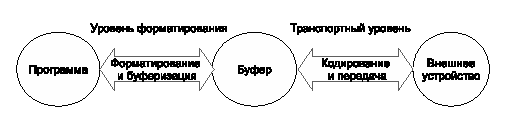
\includegraphics[width=0.7\textwidth]{img/ris_10_3}
\caption{Модель потокового ввода-вывода в \Sys{С++}}
\label{ch10:refDrawing2}
\end{center}
\end{figure}

При этом представление данных в программе и на внешнем устройстве может  отличаться: по необходимости данные могут
отображаться в форме, удобной для восприятия человеком, либо преобразовываться в какой-либо формат обмена данными. Как
видно из рисунка, собственно обработка текстовых данных выполняется на двух уровнях:
\emph{форматирования} и \emph{транспортном}. Под форматированием понимается
преобразование внутренних данных программы в человеко-читаемую последовательность символов. Например, значение
целочисленной или вещественной переменной на этом этапе должно быть преобразовано в последовательность цифр, а
управляющие символы в строковых данных должны быть заменены соответствующими им символьными последовательностями
(например, код табуляции <<\Sys{{\textbackslash}t}>> превращается в заданное число пробелов). Под
кодированием понимается трансляция из одной кодировки символов в другую. Например, транспортный уровень может выполнять
преобразование символов в кодировку Unicode для их использования за пределами программы (данная кодировка является
стандартом де-факто, но неудобна для непосредственного использования в программе,  т.~к. символы разных языков имеют в
ней различное количество байт).

В рамках двухуровневой модели ввода-вывода, принятой в \Sys{C++}, 
уровень форматирования делает возможным выполнение следующих
процедур:

\begin{itemize}
\item преобразование вещественных значений в последовательность цифр с заданной точностью и формой представления;
\item преобразование целочисленных значений в последовательность цифр в шестнадцатеричной, восьмеричной либо десятичной
системе счисления;
\item исключение лишних пробелов из входных данных;
\item задание ширины поля (т.~е. максимального количества знаков) для выводимых данных;
\item адаптация представления чисел к конкретной локали (т.~е. учёт национальной специфики их отображения).
\end{itemize}
Транспортный уровень отвечает непосредственно за получение и выдачу символов. На этом уровне инкапсулируется специфика
конкретных внешних устройств. К числу таковых помимо возможности преобразования в многобайтные кодировки относится
также блочный вывод в файлы с использованием системных вызовов операционной системы, под которую компилируется
программа.

 Для уменьшения числа обращений к внешнему устройству используется потоковый буфер. При выводе последовательность
символов после форматирования попадает в потоковый буфер, а реальная передача данных внешнему устройству выполняется
когда буфер оказывается заполнен, или когда принудительно вызвана операция опустошения буфера. При вводе данных
транспортный уровень считывает последовательность символов из внешнего устройства в буфер, после чего уровень
форматирования извлекает данные из буфера. Когда буфер оказывается пуст, задачей транспортного уровня является его
повторное наполнение данными.

Реализованный в \Sys{C++} форматированный потоковый ввод-вывод можно разделить на две группы: \emph{файловый 
ввод-вывод} и \emph{ввод-вывод в памяти}. Файловый ввод-вывод предполагает передачу данных между
программой и внешним устройством. При этом внешнее устройство только представлено файлом; помимо обычного файла на
диске оно может в действительности быть каналом обмена данными или любым реальным устройством, файловая абстракция
которого реализована в операционной системе. 

Ввод-вывод в памяти в действительности не задействует никакого внешнего устройства. Благодаря этому отпадает
необходимость в уровне кодирования и передачи, а уровень форматирования просто формирует строку символов. 

Расширяемость библиотеки потокового ввода-вывода позволяет программисту добавлять свои элементы на любом из её уровней.
Например, операторы ввода-вывода могут быть перегружены для новых типов данных, программист может создавать собственные
элементы, управляющие форматированием (т.~н. манипуляторы). Можно создавать собственные локали для специфического
представления чисел и~т.~д. 

Теперь мы можем рассмотреть, как выглядит иерархия классов потокового ввода-вывода с точки зрения программиста. 

Мы будем рассматривать упрощённое представление для случая, когда символы представлены в программе в однобайтной
кодировке с использованием типа \Sys{char}. В реальности библиотека \Sys{iostream}
реализует более универсальное представление данных на основе \emph{шаблонов}, позволяющее не
указывать заранее при описании классов тип данных, используемый для хранения символа. Благодаря этому подходу тот же
самый код может применяться, например, для многобайтных кодировок, представленных специальным типом
\Sys{wchar\_t}. Также мы на данном этапе опустим специальные средства обработки ошибок и других
исключительных ситуаций, применённые в данной библиотеке. Подробнее о шаблонах и обработке исключительных ситуаций
можно будет узнать в следующих разделах; там же будут пояснены опущенные на данном этапе элементы, и в т.~ч. то, как на
самом деле объявлены типы библиотеки \Sys{iostream}. 

Пока достаточно знать, что иерархия классов \Sys{iostream} \emph{выглядит}
 для программиста, использующего обычные символы типа \Sys{char}, следующим образом (см. рис.~\ref{ch10:refDrawing3}).

Из приведённой иерархии можно заметить, что структура классов уровня форматирования заметно более разветвлённая, хотя
основные отличия между файловыми потоками и потоками в памяти кроются на транспортном уровне. Кажущийся дисбаланс легко
объясним, если вспомнить, что программист, пользующийся библиотекой \Sys{iostream}, непосредственно
взаимодействует в основном с уровнем форматирования. Использование универсальных классов, которые после существенной
предварительной настройки выполняли бы ввод-вывод с любыми объектами транспортного уровня, менее удобно, чем
специализированные классы для каждого типа ввода-вывода, не требующие или почти не требующие настройки для выполнения
требуемых операций.

Будучи базовым для всех потоковых классов уровня форматирования, класс \Sys{ios} содержит информацию,
присущую любым потокам: управляющую информацию для разбора и форматирования, возможности для расширения иерархии
собственными потоками пользователя, а также локали. Здесь же объявляются некоторые типы, используемые остальными
классами: флаги форматирования, биты состояния, режим открытия и т.~д. Здесь же содержится указатель на потоковый буфер
(который в свою очередь включает собственно символьный буфер и служебную информацию, отражающую состояние буфера и
обеспечивающую целостность информации).

Как читатель успел заметить из собственной практики программирования на \Sys{C++}, активнее всего потоки используются для
стандартного ввода-вывода (т.~е. ввода с клавиатуры и вывода на дисплей). Для обработки стандартного ввода предусмотрен
класс \Sys{istream},  а для обработки стандартного вывода --- \Sys{ostream}; оба класса
наследуются от \Sys{ios}, приобретая благодаря этому всю специфику, связанную с форматированием, и
указатель на потоковый буфер. Для взаимодействия с потоковым буфером в классе \Sys{istream} объявлен
перегруженный оператор потокового ввода \Sys{{>}{>}}, а в классе
\Sys{ostream} --- перегруженный оператор потокового вывода \Sys{{<}{<}}.
Для возможности неформатированного ввода и вывода в этих классах объявлен также ряд методов --- таких как 
\Sys{read()} и \Sys{write()}. Наконец, для случаев, когда необходим  двунаправленный
ввод-вывод (по аналогии с тем, как файл может открываться одновременно для чтения и записи) с помощью множественного
наследования от этих двух классов порождён класс \Sys{iostream}, автоматически приобретающий свойства
как входных, так и выходных потоков и используемый как базовый для классов, в которых двунаправленный ввод-вывод
действительно востребован.

\begin{figure}[htb]
\begin{center}
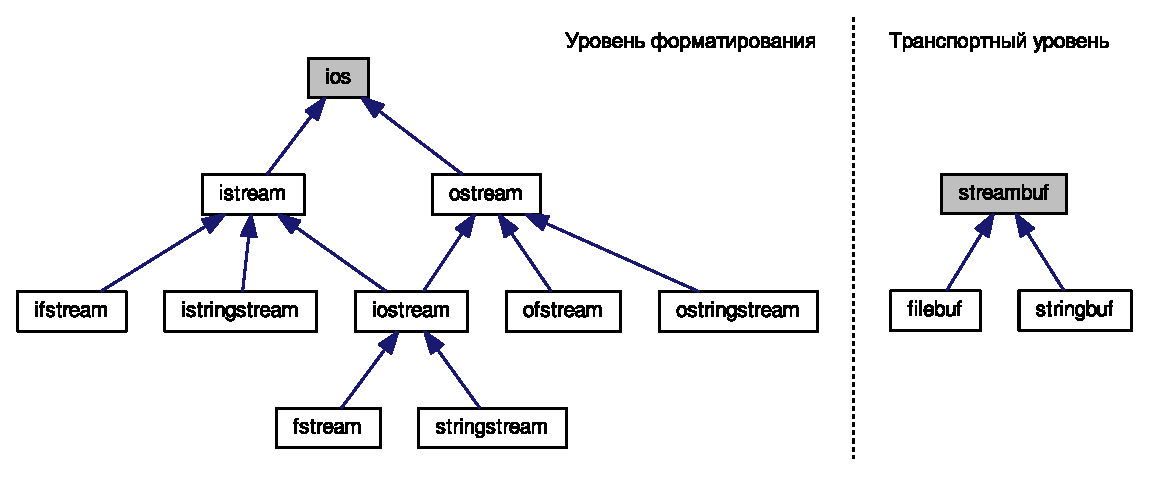
\includegraphics[width=0.7\textwidth]{img/ris_10_4}
\caption{Иерархия классов потокового ввода-вывода}
\label{ch10:refDrawing3}
\end{center}
\end{figure}

Строковые потоки, осуществляющие ввод-вывод в памяти, представлены классами \Sys{istringstream} и
\Sys{ostringtstream}, порождёнными соответственно от \Sys{istream} и
\Sys{ostream}, а также универсальным классом двунаправленного ввода-вывода
\Sys{stringtream}, порождённым от \Sys{iostream}. Эти классы включают функции (геттеры
и сеттеры) для использования строки в качестве буфера.

Файловый ввод-вывод осуществляют классы \Sys{ifstream} и \Sys{oftstream}, порождённые
соответственно от \Sys{istream} и \Sys{ostream}, а также универсальный класс
\Sys{fstream}, порождённый от \Sys{iostream}. Эти классы содержат методы для открытия и
закрытия файлов, аналогичные функциям \Sys{fopen()} и \Sys{fclose()} языка \Sys{С}.

Очевидно, что значительная часть различий между стандартным вводом-выводом, файловыми и строковыми потоками скрыта на
транспортном уровне.

Базовый класс \Sys{streambuffer} олицетворяет собой универсальный потоковый буфер. Будучи абстрактным
классом, он не содержит в себе специфики конкретных оконечных устройств; однако в нём объявлены две чисто виртуальные
функции: \Sys{overflow()} и \Sys{underflow()}, которые должны быть перегружены в
производных классах, чтобы выполнять действительную передачу символов между символьным буфером и конкретными оконечными
устройствами.

Класс потокового буфера поддерживает две символьные последовательности: область получения (\Sys{get}),
представляющую последовательность символов, получаемых из оконечного устройства, и область выдачи
(\Sys{put}), т.~е. выходную последовательность для записи на устройство. Также в классе предусмотрены
функции, извлекающие очередной символ из буфера (\Sys{sgetc()} и т.~д.) и помещающие очередной символ в
буфер (\Sys{sputc()} и т.~д.), которые обычно используются уровнем форматирования. Дополнительно
потоковый буфер содержит также объект локали.

Производный от \Sys{streambuf} класс \Sys{filebuf} используется для работы с файлами и
содержит для этого ряд функций, таких как \Sys{open()} и \Sys{close()}. Он также
наследует объект локали от базового класса для перекодирования между внешней и внутренней кодировками (например, как
уже упоминалось, между кодировкой Unicode и внутренним представлением мультиязычных символов значениями типа
\Sys{wchar\_t}).

Класс \Sys{stringbuf} также является производным от \Sys{streambuf}. Поскольку он
предназначен для работы со строками, внутренний буфер одновременно является и оконечным устройством.  По мере
необходимости внутренний буфер может динамически изменять свой размер, чтобы принять все записанные в него символы.
Класс позволяет получить копию внутреннего буфера, а также скопировать в него строку.

Взаимодействие между уровнем форматирования и транспортным уровнем осуществляется следующим образом. Класс
\Sys{ios}, как мы уже упоминали, содержит в себе указатель на потоковый буфер. В производных от него
классах (таких как \Sys{fstream} или \Sys{stringstream}) содержатся указатели на
объекты соответствующих классов транспортного уровня (\Sys{filebuf} или
\Sys{stringbuf}). Классы транспортного уровня можно также использовать и непосредственно, для
неформатированного ввода-вывода --- точно так же, как их использует уровень форматирования.

Представленная на рисунке иерархия могла бы быть описана следующим образом: 
\begin{lstlisting}
class ios {...};
class ostream : public ios{...};
class istream : public ios{...};
class ofstream : public ostream{...};
class ifstream : public istream{...};
class ostringstream : public ostream{...};
class istringstream : public istream{...};
class iostream : public ostream, public istream {...};
class fstream : public iostream{...};
class stringstream : public iostream{...};
\end{lstlisting}

\section[Обработка исключений]{Обработка исключений}
\subsection[Общие понятия]{Общие понятия}
Классический подход к обработке ошибок в программе, разработанной в рамках процедурного подхода, предполагает анализ
значений, возвращаемых функциями. Например, многие библиотечные функции в случае возникновения ошибки или какой-либо
непредвиденной ситуации возвращают нулевое значение, интерпретируемое как <<ложно>>, а в случае успешной работы ---
ненулевое, т.~е. <<истина>>. При необходимости передачи более детальной информации об ошибке, код ошибки может
сохраняться в некую глобальную переменную (библиотечные функции, унаследованные из языка С,  для этой цели используют
глобальную переменную \Sys{errno}).

У этого подхода есть два существенных недостатка. Во-первых, он не поощряет программиста проверять, была ли корректной
работа вызванной функции. Фактически, наоборот: программа, в которой половина вызовов функции обернуты условным
оператором, анализирующим возвращаемое значение, выглядит менее стройной и хуже читается из-за насыщенности однотипными
конструкциями, не имеющими отношения к основному алгоритму работы. По этой причине программисту инстинктивно хочется
выполнять проверку корректности работы как можно реже, что повышает вероятность неотслеживаемых сбоев в работе
создаваемого программного продукта. 

Второй недостаток связан с крайней лаконичностью информации об ошибке, передаваемой стандартными средствами. Например,
по коду ошибки, возникшей где-то на одном из внутренних уровней вложенности, программа определяет проблему с открытием
файла, и выдаёт пользователю сообщение <<файл не найден>>. Однако если бы механизм обработки ошибок позволял программисту
для каждого типа ошибочной ситуации стандартными средствами передавать произвольную дополнительную информацию, было бы
гораздо проще организовать информативные сообщения в духе <<не найден файл такой-то>>, или <<не удалось создать файл
такого-то размера>>, или <<выделение в памяти такого-то количества байт завершилась неудачей>>. 

Для решения этих проблем в \Sys{C++} был включён новый механизм --- \emph{обработка исключительных ситуаций}.

Исключительная ситуация (англ. <<exception>>) или \index{Исключение}\emph{исключение} --- это что-то особенное
или ненормальное, случившееся в работе программы. Чаще всего исключение --- это какая-то возникшая ошибка, но не
обязательно: например, это может быть нестандартное стечение обстоятельств или просто ситуация, требующая нетиповой
обработки.

Если в программе (или в библиотечной функции, которую использует программа) возникает какая-то неразрешимая ситуация, то
\emph{генерируется исключение}. Это означает, что вместо нормального продолжения программы
управление передаётся на другую ветку алгоритма, специально предназначенную для обработки такой исключительной
ситуации. Эта другая ветвь программы --- \index{Исключение!обработчик}\emph{обработчик исключения}
--- может просто прервать программу, а может что-то изменить, чтобы программа могла продолжить выполнение. Причём, даже
если исключение возникает в библиотечной функции,  обработчик исключения всё равно находится в программе, использующей
эту библиотеку --- в той части кода,  которая непосредственно вызвала конкретную нестандартную ситуацию и потому лучше
может справиться с её обработкой.

Чтобы исключение, сгенерированное в одном блоке кода, могло найти нужный обработчик, находящийся в другом блоке, при
генерации исключения \emph{выбрасывается}\index{Исключение!индикатор}
 \emph{индикатор исключения}. Индикатором служит объект или переменная
некоторого конкретного типа. При возникновении исключения будет выбран тот обработчик, в описании которого указан тот
же тип ожидаемого индикатора. Обработчики различают исключения по типам данных индикатора, и поэтому в наиболее
распространённом случае в качестве индикатора указывают объект некоторого класса, специально предусмотренного для этой
цели.

Программист, желающий использовать исключения, должен поместить вызов кода, в котором исключение может возникнуть, в
специальный блок \Sys{try\{\}}. Следом за этим блоком должен следовать блок
\Sys{catch()\{\}}, внутрь которого помещают код, обрабатывающий исключительную ситуацию. Например, если
исключение может возникнуть в некой функции \Sys{f()}, для его обработки нужно написать следующую
конструкцию:
\begin{lstlisting}
f() 
{
  //`генерируем исключение, если возникла соответствующая ситуация`
  if (....) throw `\Sys{индикатор}`;
  .....
}	
.....
try 
{
  //`\Sys{вызываем код, который может сгенерировать исключение}:`
  f();
}
catch(`\Sys{индикатор}`) 
{
  //`\Sys{обрабатываем исключение}`
  .....
}
\end{lstlisting}

Обработчик исключения всегда следует сразу за блоком \Sys{try\{\}}. В круглых скобках после
\Sys{catch} указывается индикатор исключения, которое этот блок обрабатывает. Чтобы сгенерировать
исключение, нужно использовать специальную конструкцию \Sys{throw}, после которой указывается
индикатор. 

В следующем примере, показывающем, как можно применить обработку исключений для организации диалогового режима работы,
мы объявим два пустых класса для использования в качестве индикаторов: класс \Sys{unknown\_exception},
означающий получение неизвестного ответа от пользователя, и класс \Sys{abort\_exception},
сигнализирующий о необходимости немедленного выхода из программы.  Сама программа задаёт пользователю вопрос о
выполнении последовательно 100 неких абстрактных пронумерованных команд. Диалог реализуется функцией
\Sys{confirm()}, спрашивающей у пользователя подтверждение на выполнение команды с заданным номером и
анализирующей ответ ('\Sys{y}' --- подтверждение, '\Sys{n}' --- отказ,
'\Sys{a}' --- немедленный выход).
\begin{lstlisting}
#include <iostream>
#include <math.h>
using namespace std;
class unknown_exception{};
class abort_exception{};
bool confirm(int i) 
{
  char c;
  cout << "`\Sys{Подтвердите команду }`" << i << " (y/n/a - `\Sys{да/нет/выход}`): ";
  cin >> c;
  cin.ignore(); //`\Sys{очищаем буфер если введены лишние символы}`
  switch (c) {
  case 'y': return true;
  case 'n': return false;
  case 'a': throw abort_exception();
  default: throw unknown_exception();
  }
}
main() 
{
  cout << "`\Sys{Демонстрация диалога подтверждения при выполнении}`"<<" 100 `\Sys{команд}`\n";
  for (int i=1;i<=100;i++) {
  try{ 
    if (confirm(i)) cout << "`\Sys{КОМАНДА}` "<< i <<"`\Sys{ ВЫПОЛНЕНА}`\n";
    else cout << "`\Sys{КОМАНДА}` " << i << " `\Sys{ОТМЕНЕНА}`\n";
  }
  catch(unknown_exception) {
    cout << "`\Sys{Неизвестный ответ пользователя}`\n";
    i--; // `возвращаемся к предыдущей команде`
  }
  catch(abort_exception) {
    cout << "`\Sys{Выполняется немедленный выход из программы}`\n";
    return 0;
  }
  cout << "`\Sys{Продолжение демонстрации диалога}`\n";
  }
}
\end{lstlisting}

Как видно из примера, обработчики исключений должны следовать друг за другом каждый в своём блоке
\Sys{catch()}. После того, как отработает один из обработчиков, управление  передастся на код,
следующий за последним блоком \Sys{catch()} в данной цепочке.

Обратите внимание, что в блоке \Sys{catch() }мы указали в качестве параметра только тип данных ---
класс-индикатор. Это допустимо с учётом того, что обработчик исключения не собирается извлекать никаких данных из
переданного индикатора, да и сами классы-индикаторы, созданные в программе, являются пустыми и используются только для
того, чтобы различать исключительные ситуации.

\subsection[Передача информации в обработчик]{Передача информации в обработчик}\label{ch10:4.2}
Как уже упоминалось, чтобы  передать в обработчик дополнительную информацию, нужно
принимать в блоке \Sys{catch()} не тип данных, а переменную. Перед выбрасыванием исключения можно её
проинициализировать конкретными данными, а потом прочитать эти данные в обработчике. 

Приведём в качестве иллюстрации ещё один пример, в котором реализован класс \Sys{array}, предоставляющий
пользователю массив с возможностью добавления и удаления элементов в стиле работы со стеком. Для этого класса будет
перегружен оператор индекса \Sys{[]}, возвращающий значение элемента с заданным номером, а также две
функции для изменения размера массива: \Sys{push()}, позволяющая добавить новый элемент в конец
массива, и \Sys{pop()}, забирающая из массива последний добавленный элемент. При создании объекта для
массива будет резервироваться память, для чего конструктору будет передаваться параметр \Sys{capacity} 
--- ёмкость массива, т.~е. максимально допустимое число элементов. 
\begin{lstlisting}
#include <iostream>
#include <math.h>
using namespace std;
class general_error 
{
public:
  char *message;
  general_error(char* message) { this->message=message; }
};
class out_of_range 
{
public:
  size_t i;
  out_of_range(size_t i) { this->i=i; }
};
class overflow {};
class underflow {};
class array 
{
  size_t size; //`реальный размер массива` 
  size_t capacity; //`максимально-допустимый размер`
  double *data;
public:
  array(size_t capacity);
  ~array();
  double operator[](size_t i); //`получить значение i-го элемента`
  void push(double v); //`добавить элемент`
  double pop(); //`убрать последний добавленный элемент` 
};
array::array(size_t capacity) 
{
  if (capacity==0) 
throw general_error("`\Sys{массив нулевой вместимости}`");
  this->capacity=capacity;
  size=0;
  data = new double[capacity];
}
array::~array() 
{
  delete[] data;
}
double array::operator[](size_t i) 
{
  if (i < size) return data[i];
  else throw out_of_range(i);
}
void array::push(double v) 
{
  if (size < capacity) data[size++]=v;
  else throw overflow();
}
double array::pop() 
{
  if (size > 0) return data[--size];
  else throw underflow();
}
main() 
{
  char c;
  size_t i;
  double v;
  cout << "`\Sys{Введите ёмкость массива: }`";
  cin >> v;
  array a(v);
  for (;;) 
  {
    cout << "`\Sys{Введите}` \"+\" `\Sys{для добавления элемента,}`" " \"-\" `\Sys{для извлечения}`, \"i\" `\Sys{для просмотра}` " "i`\Sys{-го элемента}`, \"a\" `\Sys{для выхода: }`";
    cin >> c;
    try 
    {
      switch (c) 
      {
      case '+':
	cout << "`\Sys{Введите добавляемое число: }`";
	cin >> v;
	a.push(v);
	break;
      case '-':
	v=a.pop();
	cout << "`\Sys{Извлечено число }`" << v << endl;
	break;
      case 'i':
	cout << "`\Sys{Введите индекс: }`";
	cin >> i;
	v=a[i];
	cout << "`\Sys{Искомый элемент равен }`" << v << endl; 
	break;
      case 'a':
	return 0;
	break;
      }
    }
    catch(const out_of_range& e) 
    {
      cout << "`\Sys{Попытка доступа к элементу с недопустимым индексом }`"<< e.i << endl;
    }
    catch(overflow) 
    {
      cout << "`\Sys{Операция не выполнена, так как массив переполнен}`\n";
    }
    catch(underflow) 
    {
      cout << "`\Sys{Операция не выполнена, так как массив пуст}`\n";
    }
  }
}
\end{lstlisting}

В этом примере использованы четыре класса-индикатора исключений: \Sys{general\_error} для ошибок
неопределённого типа (класс содержит строку \Sys{message}, описывающую суть возникшей проблемы),
\Sys{out\_of\_range} для выхода индекса за границу массива (свойство \Sys{i}
предусмотрено для значения индекса), а также классы \Sys{overflow} для ошибки переполнения ёмкости
массива и \Sys{underflow} для попыток удалить элемент из пустого массива. Обработчик
\Sys{out\_of\_range} принимает объект класса-индикатора и сообщает пользователю, какое именно значение
индекса оказалось недопустимым. Диалог с пользователем ведётся в бесконечном цикле, на каждой итерации которого
предлагается выбрать одно из четырёх действий: добавление элемента, удаление элемента, просмотр элемента с заданным
индексом или выход из программы. 

\subsection[Иерархия исключений]{Иерархия исключений}
Классы-индикаторы исключения могут принадлежать к общей иерархии наследования, т.~е. быть в отношениях
<<родитель-потомок>>. При этом обработчики индикаторов-родительских классов могут перехватывать исключения с
индикаторами-потомками (можно считать такое поведение проявлением полиморфизма). Поэтому родительские обработчики нужно
обязательно указывать \emph{после} дочерних в цепочке блоков \Sys{catch} --- иначе
дочерний обработчик никогда не получит управление. В самом конце цепочки можно указать \Sys{catch}, у
которого в круглых скобках вместо индикатора три точки. Такой блок будет перехватывать абсолютно любые исключения:
\begin{lstlisting}
class general_error{};
class out_of_range: public general_error {};
..............
try { ...............}
catch (out_of_range) 
{ cout << "`\Sys{Выход индекса за границу массива}`\n"; }
catch (general_error) 
{ cout << "`\Sys{Общий сбой в работе программы}`\n"; }
catch (...) {cout << "`\Sys{Неизвестная ошибка}`\n"; }
\end{lstlisting}

В приведённом схематичном примере мы объявили два различных класса-индикатора, один базовый, для исключений общего типа,
и один производный от него, для исключительной ситуации типа <<недопустимый индекс при обращении к в массиву>>. Если бы
порядок следования обработчиков был другим, обработчик индикатора \Sys{out\_of\_range} никогда не смог
бы активироваться.

Если обработчик перехватил исключение, но обнаружил, что не сможет справиться с его обработкой, он может вызвать
\Sys{throw} без аргументов: это передаст исключение дальше по цепочке уровней вложенности, на случай
если на более высоком уровне есть обработчик, способный так или иначе решить возникшую ситуацию. Проиллюстрируем
повторное возбуждение исключения, изменив пример из п.~\ref{ch10:4.2}. Цикл обработки событий мы поместим в отдельную функцию
\Sys{main\_loop()}, принимающую в качестве аргумента ссылку на массив. Соответственно, создание объекта
массива и передачу его в цикл обработки событий поместим в ещё один блок \Sys{try}, с обработчиком,
принимающим исключение типа \Sys{general\_error}.  В первую очередь это позволит корректно обрабатывать
ошибку нулевой ёмкости массива. Для иллюстрации передачи повторно сгенерированного исключения из внутреннего
обработчика внешнему специально добавим инструкцию \Sys{throw} без аргументов в обработчик события 
\Sys{out\_of\_range} (таким образом, выход индекса за границу массива станет фатальной ошибкой,
приводящей к остановке программы). Чтобы исключение могло быть успешно перехвачено на внешнем уровне вложенности,
сделаем класс \Sys{general\_error} родительским для остальных классов-индикаторов исключений.
\begin{lstlisting}
#include <iostream>
using namespace std;
class general_error 
{
public:
  char *message;
  general_error(char* message) { this->message=message; }
};
class out_of_range : public general_error 
{
public:
  size_t i;
  out_of_range(size_t i);
};
out_of_range::out_of_range(size_t i)
  :general_error("`\Sys{Выход индекса за границу массива}`") 
{ this->i=i; }
class overflow : public general_error 
{
public:
  overflow();
};
overflow::overflow():general_error("`\Sys{Переполнение массива}`") {}
class underflow : public general_error 
{
public:
  underflow();
};
underflow::underflow():general_error("`\Sys{Массив пуст}`") {}
class array 
{
  size_t size;     //`реальный размер массива`
  size_t capacity; //`максимально-допустимый размер`
  double *data;
public:
  array(size_t capacity) throw (general_error);
  ~array();
  double operator[](size_t i) throw (out_of_range); //`получить значение i-го элемента`
  void push(double v) throw (overflow); //`добавить элемент`
  double pop() throw (underflow); //`убрать последний добавленный элемент` 
};
array::array(size_t capacity) throw (general_error) 
{
  if (capacity==0) throw 
general_error("`\Sys{массив нулевой вместимости}`");
  this->capacity=capacity;
  size=0;
  data = new double[capacity];
}
array::~array() {
  delete[] data;
}
double array::operator[](size_t i)throw (out_of_range) 
{
  if (i < size) return data[i];
  else throw out_of_range(i);
}
void array::push(double v) throw (overflow) 
{
  if (size < capacity) data[size++]=v;
  else throw overflow();
}
double array::pop() throw (underflow) 
{
  if (size > 0) return data[--size];
  else throw underflow();
}
void main_loop(array& a) 
{
  char c;
  double v;
  size_t i;
  for (;;) 
  {
    cout << "`\Sys{Введите}` \"+\" `\Sys{для добавления элемента}`,"
      " \"-\" `\Sys{для извлечения}`, \"i\" `\Sys{для просмотра}` "
      "i`\Sys{-го элемента}`, \"a\" `\Sys{для выхода:}` ";
    cin >> c;
    try {
      switch (c) {
      case '+':
	cout << "`\Sys{Введите добавляемое число: }`";
	cin >> v;
	a.push(v);
	break;
      case '-':
	v=a.pop();
	cout << "`\Sys{Извлечено число }`" << v << endl;
	break;
      case 'i':
	cout << "`\Sys{Введите индекс: }`";
	cin >> i;
	v=a[i];
	cout << "`\Sys{Искомый элемент равен }`" << v << endl; 
	break;
      case 'a':
	return;
	break;
      }
    }
    catch(out_of_range& e) 
    {
      out << "`\Sys{Попытка доступа к элементу с недопустимым индексом }`" << e.i << endl;
      throw;
    }
    catch(overflow) 
    {
      cout<<"`\Sys{Операция не выполнена, так как массив переполнен}`\n";
    }
    catch(underflow) {
      cout << "`\Sys{Операция не выполнена, так как массив пуст}`\n";
    }
  }
}
main() 
{
  double v;
  try 
  {
    cout << "`\Sys{Введите ёмкость массива: }`";
    cin >> v;
    array a(v);
    main_loop(a);
  }
  catch(general_error& e) 
  {
    cout << "`\Sys{Произошла неустранимая ошибка следующего типа: }`" << e.message << endl;
  }
}
\end{lstlisting}

\subsection[Спецификация исключений]{Спецификация исключений}
Если некоторая функция содержит инструкции \Sys{throw}, в её заголовке можно явно прописать, какие
исключения она может генерировать:

\Sys{void f() throw (x,y,z);}

В примере функция \Sys{f()} может генерировать исключения с классами-индикаторами
\Sys{x, y, z} (и производными от них). Если заголовок описан как <<\Sys{void f() throw
()}>> --- функция не генерирует исключений вообще. И, наконец, если в заголовке функции ничего не указано, она может
генерировать любые исключения (без этого последнего правила не смогли бы работать программы, не использующие обработку
исключений).

Если функция попытается сгенерировать исключение, отсутствующее в её списке --- вызовется специальная функция
\Sys{void unexpected()}, которая в свою очередь вызовет фунцкию \Sys{void terminate()},
а та вызовет функцию \Sys{abort()}, аварийно завершающую программу. Программист имеет возможность
заменить функцию \Sys{unexpected()} или функцию \Sys{terminate()} --- или сразу обе --- на
свои собственные, изменив таким образом обработку неспецифицированных исключений. Для такой замены нужно вызвать
специальные библиотечные функции \Sys{set\_unexpected()} и \Sys{set\_terminate()},
передав им адреса новых функций в качестве аргументов. Наглядно можно увидеть действие этих функций в примере из
раздела 10.4.2, в котором не перехватывается исключение \Sys{general\_error}. Это исключение
выбрасывается в примере конструктором класса \Sys{array} в том случае, если пользователь попытается
создать массив нулевой ёмкости. Оно оказывается необработанным, т.~к. создание массива находится за пределом блока
\Sys{try}. К сожалению, стандартная функция не может знать о структуре класса-индикатора, и потому
текстовое сообщение, оставленное конструктором, оказывается невостребованным. Программа сообщает имя неперехваченного
класса-индикатора, после чего выполняет аварийное завершение работы.

\subsection[Стандартные классы --- индикаторы исключений]{Стандартные классы --- индикаторы исключений}
Стандартная библиотека \Sys{C++} содержит иерархию стандартных классов-индикаторов исключений (рис.~\ref{ch10:refDrawing4}),
объявленных в заголовочном файле \Sys{stdexcept}. Эти индикаторы можно использовать в собственных
программах.

\begin{figure}[htb]
\begin{center}
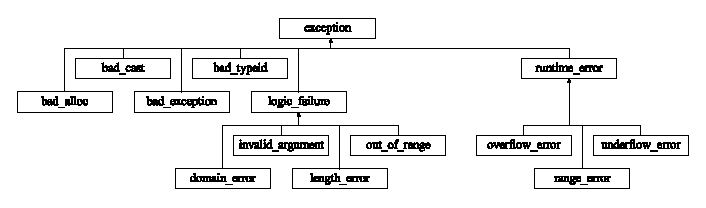
\includegraphics[width=\textwidth]{img/ris_10_5}
\caption{Предопределённые индикаторы исключений}
\label{ch10:refDrawing4}
\end{center}
\end{figure}

Назначение каждого класса-индикатора представлено в табл.~\ref{ch10:refTable2}.

\begin{longtable}{|l|p{0.65\textwidth}|}
\caption{Стандартные классы-индикаторы исключений}\label{ch10:refTable2}\\
\hline
\Emph{Исключение} &\Emph{Описание}\\
\hline \hline
\endfirsthead
\multicolumn{2}{c}%
{{\tablename\ \thetable{} --- продолжение}} \\
\hline
\Emph{Исключение} &\Emph{Описание}\\
\hline \hline
\endhead
\Sys{exception} &базовый класс для всех стандартных исключений \Sys{C++} \\\hline
\Sys{bad\_alloc} &неудача выделения памяти; может генерироваться оператором \Sys{new}\\\hline
\Sys{bad\_cast} &ошибка динамического приведения типов, генерируется \Sys{dynamic\_cast}\\\hline
\Sys{bad\_exception} &предназначено для обработки непредусмотренных исключений в программе\\\hline
\Sys{bad\_typeid} &генерируется оператором \Sys{typeid }(оператор, возвращающий имя типа, которому принадлежит аргумент),
если не удаётся определить тип объекта\\\hline
\Sys{logic\_error} &исключение, связанное с ошибкой в логике работы программы, которая, теоретически, может быть обнаружена при чтении
кода\\\hline
\Sys{domain\_error} &генерируется при выходе из математической области допустимых значений\\\hline
\Sys{invalid\_argument} &генерируется при получении недопустимого аргумента\\\hline
\Sys{length\_error} &генерируется при попытке создания слишком длинной строки\\\hline
\Sys{out\_of\_range} &выход индекса за допустимую границу\\\hline
\Sys{runtime\_error} &исключение, связанное с ошибкой, которая, теоретически, не может быть обнаружена при чтении кода\\\hline
\Sys{overflow\_error} &генерируется при обнаружении математического переполнения\\\hline
\Sys{range\_error} &генерируется при попытке сохранить значение, выходящее за границы допустимого диапазона\\\hline
\Sys{underflow\_error} &генерируется при математической ошибке исчезновения порядка\\\hline
\end{longtable}

Базовый класс \Sys{exception} содержит конструктор по умолчанию, конструктор копирования, деструктор,
перегруженный оператор присваивания, а также единственный метод \Sys{what()}, возвращающий
ASCIIZ-строку с человеко-читаемым описанием исключительной ситуации. Классы-потомки могут добавлять к этому свой
собственный функционал, в зависимости от типа ошибок, для обработки которых они предназначены. Однако стандартные
классы-индикаторы по существу являются простыми обёртками над \Sys{exception}, ограничиваясь
возможностью указать конструктору класса-индикатора сообщение, которое должен возвращать метод
\Sys{what()}. 

Воспользуемся в следующем примере двумя стандартными классами-индикаторами: 

\begin{itemize}
\item выбрасываемым автоматически при выходе индекса за пределы строки (воспользуемся классом 
\Sys{string} из стандартной библиотеки);
\item выбрасываемым при ошибке в ходе выполнения (соответствующее исключение будем генерировать сами).
\end{itemize}
\begin{lstlisting}
#include <string>
#include <stdexcept>
#include <iostream>
using namespace std;
int main ()
{
  //`перехват выхода индекса за границу массива:`
  try 
  {
     string s("sdf");
     s.replace (100, 1, 1, 'c');
  }
  catch (out_of_range &e) 
  {
    cout << "`\Sys{Обнаружен выход индекса за границу массива: }`" << e.what () << endl;
  }
  catch (exception &e) 
  {
    cout << "`\Sys{Обнаружена ошибка неопределённого вида: }`" << e.what () << endl;
  }
  catch (...) 
  {
    cout << "`\Sys{Неизвестная ошибка}`\n";
  }  
  //`перехват ошибки, возникающей в момент выполнения:`
  try 
  {
    throw runtime_error ("`\Sys{ошибка в ходе выполнения}`");
  }
  catch (runtime_error &e) 
  {
    cout << "`\Sys{Обнаружена ошибка при выполнении программы: }`" << e.what () << endl;
  }
  catch (exception &e) 
  {
     cout << "`\Sys{Обнаружена ошибка неопределённого вида: }`" << e.what () << endl;
  }
  catch (...) 
  {
    cout << "`\Sys{Неизвестная ошибка}`\n";
  }       
  return 0;
}
\end{lstlisting}

В первом случае исключение с индикатором \Sys{out\_of\_range} генерируется автоматически, когда мы
допускаем выход индекса за границу строки (такая возможность реализована классом \Sys{string} из
стандартной библиотеки). Во втором случае исключительную ситуацию с индикатором \Sys{runtime\_error}
(обозначающим ошибку, возникающую в момент выполнения программы) мы порождаем принудительно, передавая конструктору
объекта --- индикатора исключения строку с описанием подробностей. 

\section[Шаблоны классов]{Шаблоны классов}
\index{Класс!шаблон класса}Шаблоны классов во многом похожи на шаблоны функций, рассмотренные ранее. Точно так же, как и в
случае шаблонов функций, шаблоны классов позволяют отделить общий алгоритм от его реализации под
конкретные типы данных. 

Классический пример ситуации, когда выгодно применять шаблоны классов --- это так называемые контейнеры, т.~е. классы,
содержащие наборы некоторых значений (динамические списки, массивы, множества). Закладывая тип данных элемента как
параметр шаблона, можно создать универсальный класс-контейнер, а на его основе порождать объекты для хранения наборов
элементов конкретного типа --- контейнер целых чисел, контейнер строк и т.~д.

Описание шаблона класса также имеет много общего с шаблоном функции. Описание класса точно так же начинают с ключевого
слова \Sys{template}, за которым следует список формальных параметров шаблона в угловых скобках. Этот
же заголовок повторяется и перед описанием методов класса. В качестве параметров шаблона можно передавать типы данных
или константы, но перед идентификатором, обозначающим тип данных, в списке формальных параметров ставится ключевое
слово \Sys{class}.

В отличие от шаблонов функций, для которых фактические параметры шаблона (т.~е. конкретные типы данных) определяются по
типам аргументов, переданных функции, для шаблонов классов фактические параметры необходимо передавать явно. Список
фактических параметров шаблона указывается после имени класса в угловых скобках во всех случаях, когда имя шаблонного
класса используется в программе --- например, при порождении объектов, или при указании принадлежности элемента-члена
класса. Дальнейшее обращение с порождёнными объектами не отличается от обычных классов.

Рассмотрим в качестве простого примера уже знакомый класс \Sys{point}, который хранит пару координат
точки и на этот раз имеет метод \Sys{info()}, выводящий координаты на экран.
\begin{lstlisting}
#include<iostream>
using namespace std;
template <class Type> 
class point 
{
  Type x, y;
  //...
  public:
  point(Type x, Type y) { this->x=x; this->y=y; }
  void info();
};
template <class Type>
void point<Type>::info() 
{
  cout << "`\Sys{Координаты точки: }`x=" << x << ", y=" << y << endl; 
}
main()
{
  point<float> f(10.1, 20.5);
  f.info();
}
\end{lstlisting}

Как видим, конкретный тип (в нашем случае \Sys{float}) мы указали при создании объекта в угловых
скобках. Точно так же мы могли указать любой стандартный тип данных, а могли --- пользовательский тип, объявленный в
программе. Однако необходимо помнить, что шаблоны функций и шаблоны классов могут работать только для тех типов данных
(в т.~ч. классов), которые поддерживают необходимые операции. Например, если мы захотим создать экземпляр класса
\Sys{point} для хранения пары объектов какого-то собственного класса \Sys{X}, этот
класс должен содержать конструктор копирования, а также поддерживать перегрузку двух использованных в
\Sys{point} операторов:
\begin{lstlisting}
class X 
{
  ......
public:
  X(X &); //`конструктор копирования`
  friend ostream& operator<<(X &);
  .....
};
\end{lstlisting}

Как упоминалось, в качестве параметров шаблона можно передавать и константы. Рассмотрим пример, где константа передаётся
шаблонному классу \Sys{square\_matrix}, хранящему квадратную матрицу заданной размерности. Такой шаблон
позволит легко создавать объекты типов <<матрица 20х20 целых чисел>>, или <<матрица 10х10 типа
\Sys{double}>>.
\begin{lstlisting}
#include <iostream> 
using namespace std; 

template <class Type, int n> 
class square_matrix 
{ 
  Type *data; 
public: 
  square_matrix(){ data = new Type[n*n]; } 
  void print(); 
  // ... 
}; 
template <class Type, int n> 
void square_matrix<Type, n>::print() 
{ 
  for (int i=0; i<n; i++) 
  { 
    for(int j=0; j<n; j++) 
    { 
      cout << data[i*n+j] << '\t'; 
    } 
    cout << endl; 
  } 
} 
int main() 
{ 
  cout << "`\Sys{Матрица 5х5 целых чисел: }`\n"; 
  square_matrix<int, 5> m1; 
  m1.print(); 
  cout << "`\Sys{Матрица 10х10 значений типа double: }`\n"; 
  square_matrix<double, 10> m2; 
  m2.print(); 
  return 0; 
} 
\end{lstlisting}

Для простоты приведённый пример умеет только порождать матрицу заданного размера с нулевыми элементами, а также
построчно выводить её на экран.

Шаблоны классов, как и классы, поддерживают механизм наследования. Все принципы наследования при этом остаются
неизменными, что позволяет построить иерархическую структуру шаблонов, аналогичную иерархии классов.

\subsection[Типаж шаблона]{Типаж шаблона}
Иногда шаблонная функция должна реализовать нестандартное поведение для какого-либо определённого типа данных. В этом
случае в дополнение к шаблону объявляют отдельную перегруженную версию функции для нужного типа. Например, если
функция, возвращающая минимальный из двух аргументов, не может нормально работать для строковых данных, переданных
указателем на тип \Sys{char}, проблема решается так:
\begin{lstlisting}
template<class Type>
Type min(Type a, Type b) 
{
  return a<b?a:b;
}
char *min (char *a, char *b) 
{
  strcmp(a,b)<0?a:b;
}
\end{lstlisting}

С шаблонами классов может возникать аналогичная проблема, но решается она обычно несколько иначе.

Предположим, при создании шаблонного класса \Sys{matrix}, работающего с матрицами элементов
произвольного типа, оказалось, что нет возможности создать код, одинаково обрабатывающий все нужные типы данных --- т.~е.
работа некоторых методов класса \emph{должна} зависеть от типа элементов матрицы. В довершение ко всему,
типы элементов матрицы могут быть встроенными типами данных \Sys{C++}, поэтому нет никакой возможности заставить тип элемента
нести дополнительную информацию об особенностях его обработки. В результате написать единственный шаблонный класс
оказывается невозможно, а его переписывание под каждый конкретный тип данных возможно, но по определению лишено смысла:
\begin{lstlisting}
template <class Type>
class matrix 
{
  // ...
};
template<>
class matrix<long> 
{
  // ...
};
template<>
class matrix<int> 
{
  // ...
};
...
\end{lstlisting}

Фактически это означает несколько раз переписать класс заново.

Ситуация ещё более осложняется, если разработчик класса хочет оставить возможность для использования в нём новых типов
элементов (без переписывания класса с нуля).

В такой ситуации всё, что зависит от изменений типа данных, собирают в одном месте и называют \emph{типажом }(англ.
<<trait>>). Типаж передают классу как ещё один параметр шаблона.  Типаж является небольшим по объёму классом, содержащим
все операции, зависящие от типа данных, и при необходимости его несложно переписать под нужный тип. Более того,
поскольку для большинства типов никакого специфического поведения не требуется, в типаж сам по себе может быть шаблоном
класса. В этом случае как дополнительный параметр шаблона будет передаваться шаблонный класс, основанный на том же
типе, что передан в качестве основного параметра --- кроме тех редких случаев, когда требуется реализовать специфическое
поведение:
\begin{lstlisting}
template<class Type>
class MatrixTraits 
{
  // `…`
};
template<>
class MatrixTraits<int> 
{
  // `…` 
};
template<class Type, class Traits>
class matrix 
{
  // `…`
};
`…`
matrix <int, MatrixTraits<int> > m1;
\end{lstlisting}

Как правило, члены класса-типажа являются статическими функциями, поэтому его обычно используют без создания объекта.

\subsection[Пример реальной иерархии шаблонов]{Пример реальной иерархии шаблонов}
Стандартная библиотека \Sys{C++} практически полностью построена на шаблонах и потому представляет достаточно примеров
профессионального использования данного механизма.  Рассмотрим в качестве наглядной иерархии шаблонов уже знакомые нам
классы потокового ввода-вывода.

Изначально библиотека потокового ввода-вывода действительно представляла собой такую иерархию классов, которая
изображена на рис.~\ref{ch10:refDrawing3}. Однако по мере увеличения спроса на приложения, работающие с текстом сразу на
нескольких языках, встал вопрос о поддержке кодировки Unicode, позволяющей совмещать в одной строке символы разных
национальных алфавитов. В зависимости от языка, символ в Unicode может кодироваться различным количеством байт --- от
одного до четырёх. В \Sys{C++} для поддержки таких символов существует тип \Sys{wchar\_t} (от англ. wide
characters --- <<широкие символы>>). Фактически понадобилось создать иерархию классов, аналогичную классам 
\Sys{iostream}, но работающих с типом данных \Sys{wchar\_t} вместо
\Sys{char}. В итоге библиотека \Sys{iostream} была переработана на основе механизма
шаблонов.

Классы, основанные на шаблонах, носят имена, аналогичные описанным в разделе~\ref{ch10:3.6}, с добавлением приставки
<<\Sys{basic}>> и знака подчёркивания: \Sys{basic\_ios},
\Sys{basic\_istream}, \Sys{basic\_ostream}  и т.~д. Привычные программисту имена
классов для работы с символами типа \Sys{char} (как, впрочем, и с \Sys{wchar\_t})
реализованы через подстановку имени типа в конструкции \Sys{typedef}:
\begin{lstlisting}
typedef basic_ios<char> ios;
typedef basic_ios<wchar_t> wios;
typedef basic_istream<char> istream;
typedef basic_istream<wchar_t> wistream;
......
\end{lstlisting}

Используя базовые шаблоны библиотеки, можно реализовать потоковый ввод-вывод на любом собственном типе символьных данных
вместо существующих, подставив его в качестве параметра шаблона и обеспечив работу соответствующих операторов.

Хотя по виду конструкции \Sys{typedef} может показаться, что шаблоны библиотеки потокового ввода-вывода
имеют один параметр, на самом деле это не совсем так.  Второй  параметр --- это как раз \emph{типаж }символов, т.~е.
отдельный шаблонный класс, который реализует базовые операции с символами и строками для заданного типа символов. Эти
базовые операции --- присваивание символов, копирование и сравнение их последовательностей, приведение к целому типу
и др. Данный параметр имеет значение по умолчанию, и потому может не использоваться при объявлении экземпляров шаблона.
В оригинале же шаблоны классов потокового ввода-вывода выглядят следующим образом (в виду однотипности, приведём по
одному примеру для стандартного ввода-вывода, работы с файлами и со строками):
\begin{lstlisting}
template <class charT, class traits=char_traits<charT> > basic_istream;

template <class charT, class traits=char_traits<charT> > basic_ifstream;

template <class charT, class traits = char_traits<charT>, class Allocator = allocator<charT> > basic_istringstream;
\end{lstlisting}

Именно эти потоковые шаблоны определяют на самом деле методы для разбора и форматирования, являющиеся перегруженными
версиями операторов ввода \Sys{operator{>}{>}}  и вывода
\Sys{operator{<}{<}}.

Аналогично реализованы шаблоны для потоковых буферов:
\begin{lstlisting}
template <class charT, class traits = char_traits<charT> > basic_streambuf;
template <class charT, class traits = char_traits<charT> > basic_filebuf;
\end{lstlisting}

\section[Элементы стандартной библиотеки \Sys{C++}]{Элементы стандартной библиотеки \Sys{C++}}
\subsection[Базовые понятия]{Базовые понятия}
Стандартная библиотека \Sys{C++} --- это общий набор шаблонов классов и алгоритмов, позволяющий программистам легко
реализовывать стандартные структуры данных, такие как очереди, списки и стеки.

В библиотеке выделяют пять основных компонентов:

\begin{itemize}
\item Контейнер (\Sys{container}) --- хранение набора объектов в памяти.
\item Итератор (\Sys{iterator}) --- обеспечение средств доступа к содержимому контейнера.
\item Алгоритм (\Sys{algorithm}) --- определение вычислительной процедуры.
\item Адаптер (\Sys{adaptor}) --- адаптация компонентов для обеспечения различного интерфейса.
\item Функциональный объект (\Sys{functor}) --- сокрытие функции в объекте для использования другими
компонентами.
\end{itemize}

\subsection[Контейнеры]{Контейнеры}
Будем считать, что стандартная библиотека реализует следующие \index{Контейнер}контейнеры:

\begin{itemize}
\item \Sys{vector} --- линейный массив (особенно эффективен при добавлении элементов в конец);
\item \Sys{list} --- двусвязаный список (более эффективен при вставке и перестановке элементов);
\item \Sys{set} --- ассоциативный массив уникальных ключей (математический тип множество);
\item \Sys{multiset} --- ассоциативный массив с возможностью дублирования ключей;
\item \Sys{bitset} --- массив, обеспечивающий компактное хранение заданного количества битов;
\item \Sys{map} --- ассоциативный массив с уникальными ключами и значениями (хорош при поиске по ключу);
\item \Sys{multimap} --- ассоциативный массив с возможностью дублирования ключей и значений;
\item \Sys{stack} --- структура данных типа стек;
\item \Sys{queue} --- структура данных типа очередь;
\item \Sys{priorityqueue} --- очередь с приоритетами;
\item \Sys{deque} --- очередь с двухсторонним доступом.
\end{itemize}
Например, стек целых чисел можно объявить так:

\Sys{stack{<}int{>} s;}

С чуть большими затратами можно заставить работать контейнеры с собственным типом данных.

Основные методы, которые присутствуют почти во всех коллекциях стандартной библиотеки, приведены ниже.

\begin{itemize}
\item \Sys{empty} --- определяет, является ли коллекция пустой.
\item \Sys{size} --- определяет размер коллекции.
\item \Sys{begin}, \Sys{end} --- указывают на начало и конец коллекции.
\item \Sys{rbegin}, \Sys{rend} --- то же, но для желающих пройти коллекцию от конца к
началу.
\item \Sys{clear} --- удаляет все элементы коллекции (если в коллекции сохранены указатели, нужно ещё
удалить все элементы вручную вызовом \Sys{delete}).
\item \Sys{erase} --- удаляет элемент или несколько элементов из коллекции.
\item \Sys{capacity} --- вместимость коллекции определяет реальный размер --- то есть размер буфера
коллекции, а не то, сколько в нём хранится элементов. Когда вы создаёте коллекцию, то выделяется некоторое количество
памяти. Как только размер буфера оказывается меньшим, чем размер, необходимый для хранения всех элементов коллекции,
происходит выделение памяти для нового буфера, а все элементы старого копируются в новый буфер.
\item \Sys{insert} --- вставка элемента в произвольном месте последовательности
\end{itemize}
Есть также и необязательные операции: \Sys{front}, \Sys{back},
\Sys{push\_front}, \Sys{push\_back}, \Sys{pop\_front},
\Sys{pop\_back}, и оператор \Sys{[]}.

\subsection[Итераторы]{Итераторы}
Итератор (\Sys{iterator}) согласно Википедии --- объект, позволяющий программисту перебирать все элементы
коллекции без учёта особенностей её реализации. В простейшем случае итератором в низкоуровневых языках является
указатель.

В \Sys{C++} есть несколько разных типов \index{Итератор}итераторов (табл.~\ref{ch10:refTable3}):

\begin{longtable}{|p{0.35\textwidth}|p{0.55\textwidth}|}
\caption{Типы итераторов}\label{ch10:refTable3}\\
\hline
\Emph{Итератор} &\Emph{Описание}\\
\hline \hline
\endfirsthead
\multicolumn{2}{c}%
{{\tablename\ \thetable{} --- продолжение}} \\
\hline
\Emph{Итератор} &\Emph{Описание}\\
\hline \hline
\endhead
\Sys{input\_iterator} (для чтения) &
Читают значения с движением вперёд. Могут быть инкрементированы, сравнены и разыменованы.\\\hline
\Sys{output\_iterator} (для записи) &
Пишут значения с движением вперёд. Могут быть инкрементированы и разыменованы.\\\hline
\Sys{forward\_iterator} (однонаправленные) &
Читают или пишут значения с движением вперёд. Комбинируют функциональность предыдущих двух типов с возможностью
сохранять значение итератора.\\\hline
\Sys{bidirectional\_iterator} (двунаправленные) &
Читают и пишут значения с движением вперёд или назад. Похожи на однонаправленные, но их также можно инкрементировать и
декрементировать.\\\hline
\Sys{random\_iterator} (с произвольным доступом) &
Читают и пишут значения с произвольным доступом. Самые мощные итераторы, сочетающие функциональность двунаправленных
итераторов и возможность выполнения арифметики указателей и сравнений указателей.\\\hline
\Sys{reverse\_iterator} (обратные) &
Или итераторы с произвольным доступом, или двунаправленные, движущиеся в обратном направлении.\\\hline
\end{longtable}

Итераторы обычно используются парами: один для указания текущей позиции, а второй  для обозначения конца коллекции
элементов. Итераторы создаются объектом-контейнером, используя стандартные методы \Sys{begin()} и
\Sys{end()}. Функция \Sys{begin()}возвращает указатель на первый элемент, а
\Sys{end()} --- на воображаемый несуществующий элемент, следующий за последним.

К элементам контейнера --- например, \Sys{vector} --- можно обращаться и по номерам,
как к элементам классического массива --- и с помощью итераторов:

{\noindent\tabcolsep=0.1em
\begin{center}
\begin{tabular}{|p{0.44\textwidth}|p{0.54\textwidth}|}
\hline
\footnotesize\Emph{Необъектный подход} &\footnotesize\Emph{Правильный (объектный) подход}\\\hline
\begin{lstlisting}
#include <iostream>
#include <vector>
using namespace std;
main() 
{
  vector<int> a;
  //`добавляем элементы`
  a.push_back(1);
  a.push_back(4);
  a.push_back(8);
  for(int y=0;y<a.size();y++)
  {
    //`выводим 1 4 8`
    cout<<a[y]<<" ";
  }
}
\end{lstlisting}
&
\begin{lstlisting}
#include <iostream>
#include <vector>
using namespace std;
main() 
{
 vector<int> a;
 vector<int>::iterator it;
 //`добавляем элементы`
 a.push_back(1);
 a.push_back(4);
 a.push_back(8);
 for(it=a.begin();it!=a.end();it++)
 {
   //`выводим 1 4 8`
   cout<<*it<<" ";
 }
}
\end{lstlisting}
\\\hline
\end{tabular}
\end{center}
}

В отличие от счётчика цикла, итератор обеспечивает доступ к элементу, а не только его перебор. В отличие от операции
индексации, итератор <<не портится>> при добавлении в контейнер новых элементов. Кроме того, индексация иногда вообще
неприменима --- например, в коллекциях с медленным произвольным доступом, таких как списки (\Sys{list}).

Рассмотрим, как использовать контейнеры на примере класса \Sys{vector}:
\begin{lstlisting}
#include <iostream>
#include <vector>
#include <algorithm>
using namespace std;
main() 
{
  //`Объявляем вектор из целых чисел`
  vector <int> k;
  //`Добавляем элементы в конец вектора`
  k.push_back(22);
  k.push_back(11);
  k.push_back(4);
  k.push_back(100);
  vector <int>::iterator p;
  cout << "`\Sys{Вывод неотсортированного вектора:}`\n";
  for (p = k.begin(); p<k.end(); p++) {
    cout << *p << ' ';
  }
  //`Сортировка вектора.`
  sort(k.begin(), k.end());
  cout << "\n`\Sys{Вывод отсортированного вектора:}`\n";
  for (p = k.begin(); p<k.end(); p++) 
  {
    cout << *p << ' ';
  }
  cout << endl;
}
\end{lstlisting}

Как видно, пример сначала заполняет вектор целых чисел четырьмя значениями, затем поэлементно выводит содержимое вектора
на экран, сортирует с использованием \emph{алгоритма} \Sys{sort}, а затем снова выводит на
экран. Вывод программы выглядит следующим образом:
\begin{verbatim}
Вывод неотсортированного вектора: 
22 11 4 100 
Вывод отсортированного вектора: 
4 11 22 100 
\end{verbatim}

\subsection[Алгоритмы]{Алгоритмы}
В состав стандартной библиотеки входит группа функций, выполняющих некоторые стандартные действия, например поиск,
преобразование, сортировку, поштучный перебор элементов, копирование и т.~д. Они называются
\index{Алгоритм}\emph{алгоритмами}. Параметрами для алгоритмов, как правило, служат
итераторы. Алгоритму нет никакого дела до типа переданного ему итератора, лишь бы итератор подпадал под определённую
категорию. Так, если параметром алгоритма должен быть однонаправленный итератор, то подставляемый итератор должен быть
либо однонаправленным, либо двунаправленным, либо итератором произвольного доступа. 

Например, алгоритм простого поиска \Sys{find} просматривает элементы подряд, пока нужный не будет
найден. Для такой процедуры вполне достаточно итератора ввода. С другой стороны, алгоритм более быстрого бинарного
поиска \Sys{binary\_search} должен иметь возможность переходить к любому элементу последовательности, и
поэтому требует итератора с произвольным доступом.

Многие алгоритмы получают в качестве параметра различные функции. Эти функции используются для сравнения элементов, их
преобразования и т.~д. Однако вызов функции по указателю --- ресурсоёмкая операция. Вместо указателя на функцию можно
передать объект любого класса с перегруженным оператором вызова функции \Sys{operator()}. Одно из
преимуществ обращения к переопределённому оператору вызова функции вместо собственно её вызова заключается в том, что
переопределённый оператор может быть реализован в классе как встроенная функция, т.~е. код оператора будет подставлен
вместо вызова.

Рассмотрим пример алгоритма \Sys{find}, который находит первое вхождение заданного значения в коллекцию.
Алгоритм принимает в качестве аргументов пару итераторов и искомое значение; соответственно возвращается итератор,
указывающий на первое вхождение заданного значения. Благодаря универсальности механизма итераторов, алгоритм будет
работать со структурой любого типа, в том числе и с обычными массивами языка \Sys{C}. Например, чтобы найти первое вхождение
числа 7 в массив целых, требуется выполнить следующий код, использующий в качестве итераторов обычные указатели:
\begin{lstlisting}
int data[100];
...
int *where;
where = find(data, data+100, 7);
\end{lstlisting}

Поиск первого значения в целочисленном векторе выглядит приблизительно так же:
\begin{lstlisting}
vector<int> a;
...
vector<int>::iterator where;
where = find(a.begin(), a.end(), 7);
\end{lstlisting}

\section[Задачи для самостоятельного решения]{Задачи для самостоятельного решения}
\subsection[Иерархия классов]{Иерархия классов}\label{ch10:7.1}
Определить иерархию наследования из двух классов в соответствии с номером задания.
Каждый класс снабдить свойствами и методами в соответствии с предметной областью, указанной в варианте задания. В
базовом классе предусмотреть метод info(), выводящий на экран информацию об объекте. Предусмотреть конструкторы,
инициализирующие свойства объектов переданными данными либо значениями по умолчанию. Написать демонстрационную
программу, создающую 4-5 объектов и выводящую на экран информацию о них. Варианты классов:

\begin{enumerate}
\item <<Водный транспорт>>, <<Грузовое судно>>
\item <<Летательный аппарат>>, <<Дирижабль>>
\item <<Здание>>, <<Коттедж>>
\item <<Двигатель>>, <<Двигатель внутреннего сгорания>>
\item <<Устройство печати>>, <<Струйный принтер>>
\item <<Устройство ввода>>, <<Цифровая камера>>
\item <<Растровое изображение>>, <<Репродукция картины>>
\item <<Млекопитающее>>, <<Собака>>
\item <<Транспортное средство>>, <<Легковой автомобиль>>
\item <<Печатное издание>>, <<Номер журнала>>
\item <<Документ>>, <<Квитанция об оплате>>
\item <<Пищевой продукт>>, <<Йогурт>>
\item <<Корпусная мебель>>, <<Книжный шкаф>>
\item <<Проверка знаний>>, <<Экзамен>>
\item <<Носитель информации>>, <<Компакт-диск>>
\item <<Аудиозапись>>, <<файл в формате MP3>>
\item <<Видеозапись>>, <<Художественный фильм>>
\item <<Транспортное средство>>, <<Маршрутный автобус>>
\item <<Средство связи>>, <<Сотовый телефон>>
\item <<Человек>>, <<Член клуба>>
\item <<Птица>>, <<Почтовый голубь>>
\item <<Электронная карта>>, <<Абонемент на проезд>>
\item <<Дата>>, <<День рождения>>
\item <<Удостоверение>>, <<Паспорт>>
\item <<Сотрудник компании>>, <<Начальник отдела>>
\end{enumerate}
\subsection[Перегрузка операторов]{Перегрузка операторов}
Реализовать класс, содержащий коллекцию объектов, методы для включения и удаления элементов, вывода содержимого
коллекции на экран, а также перегруженный в соответствии с заданием оператор. Написать  программу, заполняющую
коллекцию несколькими элементами и демонстрирующую пользователю работу перегруженного оператора для элементов
коллекции:

\begin{enumerate}
\item <<–>> (вычитание одной коллекции из другой), класс <<множество символов>>
\item <<+>> (объединение коллекций), класс <<множество целых чисел>>
\item <<*>> (пересечение коллекций), класс <<множество целых чисел>>
\item <<!=>> (сравнение коллекций на неравенство), класс <<неупорядоченный массив вещественных чисел>>
\item <<==>> (сравнение коллекций на неравенство), класс <<упорядоченный массив символов>>
\item <<[]>> (получение элемента по его номеру в коллекции), класс <<неупорядоченный массив целых чисел>>
\item <<[]>> (получение элемента по его номеру в коллекции), класс <<упорядоченный массив вещественных чисел>>
\item <<\%>> (проверка элемента на принадлежность коллекции), класс <<множество целых чисел>>
\item <<\%>> (проверка элемента на принадлежность коллекции), класс <<упорядоченный массив символов>>
\item <<{<}{<}>> (удаление элемента из коллекции с его выводом на экран), класс <<множество целых чисел>>
\item <<{>}{>}>>  (добавление введённого с клавиатуры элемента в коллекцию), класс <<множество
символов>>
\item <<{>}=>> (проверка на включение коллекции, заданной вторым аргументом, в начальную часть коллекции,
заданной первым аргументом), класс <<упорядоченный массив символов>>
\item <<{<}=>> (проверка на включение коллекции, заданной первым аргументом, в начальную часть коллекции, заданной
вторым аргументом), класс <<неупорядоченный массив символов>>
\item <<++>> (добавление элемента со значением, на единицу больше последнего добавленного элемента), класс <<упорядоченный
массив целых чисел>>
\item <<++>> (добавление элемента со значением, на единицу больше последнего добавленного элемента), класс <<стек целых
чисел>>
\item <<-{}->> (удаление последнего добавленного элемента), класс <<упорядоченный массив целых чисел>>
\item <<-{}->> (удаление элемента), класс <<очередь вещественных чисел>>
\item <<-{}->> (опустошение коллекции), класс <<множество вещественных чисел>>
\item <<{>}{>}>>  (добавление введённого с клавиатуры элемента в коллекцию), класс <<очередь целых
чисел>>
\item <<{<}{<}>> (удаление элемента из коллекции с его выводом на экран), класс <<очередь вещественных
чисел>>
\item <<{>}{>}>>  (добавление введённого с клавиатуры элемента в коллекцию), класс <<стек символов>>
\item <<{<}{<}>> (удаление элемента из коллекции с его выводом на экран), класс <<стек целых чисел>>
\item <<*>> (умножение всех элементов коллекции на заданное число), класс <<неупорядоченный массив вещественных чисел>>
\item <</>> (деление всех элементов коллекции на заданное число), класс <<множество вещественных чисел>>
\item <<\~{}>> (смена регистра), класс <<множество символов>>
\end{enumerate}
\subsection[Обработка исключительных ситуаций]{Обработка исключительных ситуаций}
Снабдить класс из задания п.~\ref{ch10:7.1} проверкой на допустимость значений, 
передаваемых конструктору. В случае передачи
недопустимых значений генерировать исключительную ситуацию. Предусмотреть не менее двух различных классов-индикаторов
исключения, позволяющих передать обработчику необходимую информацию. 
Расширить демонстрационную программу показом
обработки некорректной инициализации объектов. 

\renewcommand{\arraystretch}{1.0}
